\documentclass[12pt]{article}

\usepackage{setspace}
\usepackage[colorlinks,urlcolor=cyan,linkcolor=,citecolor=,pdfusetitle]{hyperref}
\usepackage[margin=1in]{geometry}
\usepackage[no-math]{fontspec}

\usepackage{amsmath}
\usepackage{amssymb}
\usepackage{array}
\usepackage{caption}
\usepackage[noabbrev,nameinlink]{cleveref}
\usepackage{graphicx}
\usepackage{fancyvrb}
\usepackage{fvextra}
\usepackage[math]{kurier}
\usepackage[shortlabels]{enumitem}
\usepackage{emoji}
\usepackage{longtable}
\usepackage{luacode}
\usepackage{microtype}
\usepackage{minted}
\usepackage{multirow}
\usepackage{parskip}
\usepackage{pdflscape}
\usepackage{ragged2e}
\usepackage{sepfootnotes}
\usepackage{xfrac}

\setemojifont{TwemojiMozilla.ttf}
\renewcommand{\familydefault}{\sfdefault}

{\sf\global\expandafter\let\expandafter\lmss\the\font}
\begin{luacode}
local lmss = font.id("lmss")
local nodeprocessor = function(head)
  for n in node.traverse_glyph(head) do
    if n.char >= 48 and n.char <= 57 and n.font ~= lmss and string.sub(font.fonts[n.font].name,1,3) == "cmr" then
      n.font = lmss
    end
  end
  return head, false
end
luatexbase.add_to_callback("pre_linebreak_filter", nodeprocessor, "numbers in math mode should be sans-serif")
\end{luacode}

\setlist[itemize,1]{label=$\bullet$}
\setlist[itemize,2]{label=$\circ$}

\author{Sam Haskins}
\title{An agent- and message-based simulation framework for computer security challenges}

\fvset{breaklines=true}
\newcolumntype{R}[1]{>{\RaggedRight}p{#1}}

\renewcommand*\contentsname{Table of Contents}

\graphicspath{{figures}}

\newcommand{\subsubfigintoc}[1]{%
  \phantomsection%
  \addtocounter{figure}{1}%
  \addcontentsline{toc}{subsubsection}{Figure \thefigure: #1}%
  \addtocounter{figure}{-1}}

\newcommand{\subtabintoc}[1]{%
  \phantomsection%
  \addtocounter{table}{1}%
  \addcontentsline{toc}{subsection}{Table \thetable: #1}%
  \addtocounter{table}{-1}}

\begin{document}

\pagenumbering{roman}
\thispagestyle{empty}
\begin{center}
    \vspace*{0.9in}
    
    {\Large \textbf{An agent- and message-based simulation framework for computer security challenges} \par}
    \vspace{1in}
    
    {\large
    by \\
    \vspace{0.5in}
    \textbf{Sam Haskins}\makebox[0pt][l]{ \emoji{sparkles}} \par
    \vspace{0.9in}
    
    {
    \setstretch{1.3}
    An honours project submitted \\
    in partial\footnote{Specifically, {\normalsize \sfrac{1}{40}}\textsuperscript{th}.} fulfillment of the requirements \\
    for the degree of \\
    \textbf{Bachelor of Computer Science} \\
    }
    \vspace{0.4in}
    \textbf{Supervisor:} Dr.\@ Jason Hinek \par
    \vspace{0.6in}
    
    {
    \setstretch{1.3}
    Carleton University \\
    Ottawa, Ontario, Canada\makebox[0pt][l]{ \emoji{flag-canada}}\vspace{1.7mm} \\
    \textbf{April 18, 2025}
    }
    \par
    \vfill
    }
\end{center}

\section*{Abstract}
\addcontentsline{toc}{section}{Abstract}

Modern computer security is more than just algorithms---every day, terabytes of communications are secured with \textit{protocols} such as TLS and SSH. Flaws in these protocols can and do compromise security goals even without flaws in the underlying algorithms. Existing teaching and auto-grading tools are not suited to simulate protocols: they lack the vocabulary to express key concepts like agents and messages. This project introduces Tulila, a simulation framework and auto-grading tool where agents, networks, and messages are first-class concepts. Tulila is purpose-built to be the perfect tool for learners to explore protocol flaws hands-on and for teachers to teach and evaluate knowledge of protocol vulnerabilities. Agent behavior is defined using Python, and attack primitives such as active and passive interception are built-in, making Tulila flexible enough to simulate any protocol vulnerability or vulnerability class.

\newpage

\section*{Acknowledgements}
\addcontentsline{toc}{section}{Acknowledgements}

Special thanks to:
\begin{itemize}
  \item My supervisor, Dr.\@ Jason Hinek, for all of the illuminating discussions over the course of this project.
  \item Adrien ``doggkidd'' Boileau for drawing the banner art for Tulila.
  \item The authors of all of the third-party software libraries and content used by or included in Tulila; this is further enumerated in \cref{section:third-party-content}, below.
\end{itemize}

\newpage

\pdfbookmark[1]{Table of Contents}{Table of Contents}
\tableofcontents
\newpage

\pagenumbering{arabic}


\section{Introduction}

\sepfootnotecontent{crime}{Compression Ratio Info-leak Made Easy.}

Modern cryptography, and computer security more broadly, builds \textit{protocols}: detailed descriptions of how agents should communicate over a network, generally presented with an argument as to what security properties the protocol provides and why. Many important vulnerabilities stem from flaws in protocols or implementations, not the actual cryptographic algorithms. This category includes extremely significant vulnerabilities such as Heartbleed (I'm sure you remember the headlines) and CRIME\sepfootnote{crime} (less famous, but very fundamental and it certainly shook the cryptographic world to its core). It is important that future cryptographers and software engineers are given hands-on experience with protocols and known vulnerability categories.

At this point, I am familiar with quite a few approaches intended to give hands-on experience with cryptographic and computer security vulnerabilities. Unfortunately, these approaches are not suitable to teach vulnerabilities in protocols. Some motivating examples are:

\sepfootnotecontent{what-course-code}{COMP 2108. Previously COMP 3109, which I took, and COMP 4109.}

\begin{enumerate}
  \item I was a student and, later, a two-time teaching assistant in Dr.\@ Jason Hinek's Applied Cryptography and Authentication course\sepfootnote{what-course-code}. In this course, students were asked to complete graded cryptography challenges. Each student was given a unique, pseudo-randomly generated text file with the challenge and asked to solve it. This approach was used to give students hands-on experience with some important cryptographic vulnerabilities like one time pad re-use, insecure pseudo-random number generation, and short RSA keys. Unfortunately, this approach cannot be used to give students hands-on experience with protocols---you can't ``stuff a protocol into a text file.''
  \item I was a major contributor to the IoT (Internet of Things) Village and Embedded Systems Village Capture-the-Flags at DEF CONs 30 \& 31, respectively. (A capture-the-flag is a series of computer security challenges that end in a short string, the ``flag'', that can be submitted for points.) Here, a major focus was developing challenges using as much real-world software and hardware as possible. For example, a Heartbleed challenge in this paradigm would use a real, period-accurate version of OpenSSL and the Apache web server.
      
      This approach works, but presents some issues relevant to use in an educational setting:
      \begin{enumerate}
        \item Challenges require lots of time-consuming one-off work to develop.
        \item Challenges tend to require around-the-clock monitoring by a team of experienced professionals, including the challenge creator(s). The complexity that arises from using real software makes challenges difficult or even impossible to ``set and forget.''
        \item Most importantly, this approach introduces a lot of messy detail that isn't required, and is in fact a distraction, when teaching core concepts. For example, it's entirely possible for a student to understand CRIME and how to avoid it \textit{without} first, e.g.,  learning the intricacies of the JavaScript XMLHTTPRequest API as implemented in 2013. The extra complexity is desirable for a competition at a convention, but not so much when, e.g., teaching a second-year university course.
      \end{enumerate}
\end{enumerate}

\sepfootnotecontent{two-four-oh-six}{Fundamentals of Web Applications, COMP 2406.}

To share another anecdote, I developed a padding oracle challenge for Dr.\@ Hinek's Applied Cryptography and Authentication course. This is clearly seen as an important attack to teach students, as it has been included in every offering since I made it, but it's not the type of challenge that fits in a text file. Students must be able to send messages to a server (that has the secret key) and receive responses. It's not immediately obvious how this should be implemented; the natural way for students to send messages to a server is over HTTP, but the course in which HTTP is taught\sepfootnote{two-four-oh-six} is not a prerequisite. What to do? I ended up using HTTP anyways, but provided starter code (with a variable named \texttt{\_DO\_NOT\_TOUCH\_session}) so students could send a message by calling a function. This worked well enough for the padding oracle challenge, but this sort of approach cannot easily be extended to teach other important cryptographic vulnerabilities, including any that use the Machine-in-the-Middle attack model. Besides, how exactly messages get from Point A to Point B is an implementation detail that need not be exposed to students to teach them the concepts.

\sepfootnotecontent{saying-guide}{Pronunciation guide: about a second starting at 1:58 of \url{https://www.youtube.com/watch?v=d-nxW9qBtxQ}}

What I really wanted was a framework that let me build challenges where agents, networks, and messages were first class concepts---one where students would be able to just call \texttt{send()}, \texttt{receive()}, and \texttt{solve()}. One where it was easy to create challenges ``from whole cloth,'' with no need to ever figure out how to configure, e.g., 2013 Apache. And thus Tulila\sepfootnote{saying-guide}---my honours project---was born.

Tulila is, per the title, ``an agent- and message-based simulation framework for computer security challenges.'' Let's dig into what that means a bit more. At a high level, Tulila is software that can be installed on a server and configured to serve challenges to users over a network. In this sense, it is similar to other software used at Carleton University such as Gradescope; however, Tulila challenges offer features above and beyond those supported by Gradescope (or indeed any software that I'm aware of).

The best way to understand Tulila is to try it out yourself! (You should not be surprised that I'm saying this, as a presupposition inherent to this project is that hands-on experience is better than book learning.) You can visit Tulila at \url{https://tulila.mywire.org} and log in with the credentials ``\texttt{Imaginative-Conflict664}'' / ``\texttt{127ca733-579a-cec7-feb2-6e5c32846979}'' or, alternatively, contact me and I'll make you an account of your own. You should play through the series of 7 tutorial challenges---they can be completed with only basic Python knowledge and will give you a much better idea of what Tulila is than just reading about it. If you're cryptographically-minded, you can also try out the 3 cryptography challenges; this should give you a good idea of how to use Tulila for hands-on experience with cryptographic vulnerabilities (though do note that I don't explain how to actually solve these, I just give information on the protocol).

Now that you've completed the 7 tutorial challenges, read on---the next section formally explains what a Tulila challenge consists of. You likely already have a good idea of this from the tutorial challenges, but I will explain it here for further clarification and (mostly) for the benefit of any readers who don't know Python.

\subsection{Terminology}

The italicized terms in this section are concepts used extensively throughout the rest of this report; they are meant to be understood in the context provided here.

A Tulila \textit{challenge} is made up of a set of \textit{networks} and a set of \textit{agents}. Networks and agents are both logical objects within Tulila that are defined by the challenge author. Agents are implemented by small Python programs and may exchange structured \textit{messages} over the networks they are in, implementing one or more \textit{protocols}. (A protocol is just a set of rules for how agents generate and respond to messages.) The challenge author may grant certain agents the privilege to set one or more \textit{solution strings}; these are short strings each associated with a \textit{score}.

Every challenge has a single agent without an associated Python program providing its behavior. This agent's behavior is instead provided by the challenge recipient; they submit a Python program (the \textit{solution}) using Tulila's web interface. This starts a \textit{simulation}: every agent in the challenge is started and allowed to send and receive messages over networks. The simulation ends when a correct solution string is submitted, if an agent with permission to do so directly marks the challenge as solved, or when any agent finishes. The simulation results in a \textit{score}: a value between 0 and 1 representing how well the submission performed on the challenge. Some additional information such as lines \texttt{print()}ed is also made available to assist in debugging solutions.

To simulate real-world attack models, agents may be given elevated privileges on certain networks. These are:
\begin{enumerate}
  \item \textit{Monitor} --- the agent will receive a copy of all messages sent over the network, even those that are not addressed to it.
  \item \textit{Spoof} --- the agent may send messages that appear to come from another agent.
  \item \textit{Intercept} --- the agent may modify or drop any message sent over the network before it reaches its destination.
\end{enumerate}

Monitors correspond to passive attackers and interceptors correspond to active attackers (in the standard terms of art).

\subsection{Structure of this Report}

This report is organized into three sections (after the introduction):

\begin{enumerate}
  \item The first section is the \textit{Deployers' Guide}. This section answers the question: ``OK, I want to use Tulila. How do I do that?'' This section is the definitive guide on installing, configuring, and administering Tulila and also has some pointers on how to create Tulila challenges and how to use Tulila as part of a university course.
  \item The second section discusses Tulila's \textit{Design and Implementation}. If you're interested in knowing what makes Tulila ``tick,'' this is the section for you. A subsection of particular note contains information on the agent sandbox.
  \item The third and final section of this report enumerates the \textit{Third-Party Content} included with Tulila. Like most modern software, Tulila uses various software libraries to handle general tasks that are not unique to it, and it also includes other third-party content. This section enumerates exactly what third-party content Tulila uses or includes and who/where it's from. Information on the legal basis to use each piece of third-party content (generally a common open-source license) is included as well.
\end{enumerate}


\section{Deployers' Guide}

This section covers how to install Tulila on a server and how to complete common administrative tasks like adding challenges, creating users, and exporting scores. It will also briefly touch on how to create challenges, though the primary reference for this is the challenges that are shipped with Tulila. Some brief recommendations on how to use Tulila as part of a university course are included.


\subsection{Installing Tulila}

\textbf{Prerequisites:}\\
Tulila requires a Linux kernel with support for \href{https://www.kernel.org/doc/html/v4.17/userspace-api/seccomp_filter.html}{SECCOMP BPF} and the \href{https://docs.kernel.org/security/landlock.html}{Landlock LSM} to function. Most Linux-based operating systems released after 2021 support these by default. Tulila will not run on any other operating system kernel; no provision is made to support Windows, macOS, etc.

Root privileges are required to install Tulila.

Tulila requires \texttt{systemd} and \textit{cannot} be installed on any Linux distribution that uses a different init system. As of 2025, all widely used Linux distributions use \texttt{systemd} as their init system as it is vastly superior to its predecessor, SysVinit. To verify that your distribution uses \texttt{systemd}, run ``\texttt{command -v systemctl \&\& echo 'systemd is in use.'}''.

Aside from the init-system restriction, Tulila can be installed on any Linux distribution, and these instructions will allow you to do so. However, Tulila requires certain system-wide dependencies to be installed. These instructions, and the \texttt{install-deps.sh} script shipped with Tulila, cover installing these dependencies on Ubuntu 24.04 only. If you are installing Tulila on a server running a different distribution of Linux, information on what dependencies are required will be provided, but you must figure out how to install them by yourself. The great number and variance of Linux distributions makes it impossible to write detailed instructions for each; you are encouraged to fill in the gaps with your own knowledge.

It is recommended to set the time zone on the server to which Tulila is to be installed. This will be used by Tulila when displaying times to clients. It is likely that you set the correct time zone when installing the operating system, but this may not be the case for cloud images. The command to set the time zone on Debian, Ubuntu, and other Debian derivatives is ``\texttt{dpkg-reconfigure tzdata}''.

The text portion of these instructions generally covers \textit{what} must be done, but not necessarily \textit{how}. Whenever possible, the specific commands to run and sample output will be included verbatim underneath the text. As a convention in these verbatim sections, ``\texttt{\$}'' indicates an unprivileged shell and ``\texttt{\#}'' indicates a root shell.

\bigskip
\textbf{Step 1: Download and extract the Tulila distribution file}
\begin{enumerate}[I.]
  \item Using whatever means are convenient, download the \texttt{tulila.tar.xz} file (included alongside this report) to your server.
  \item Extract the file. As it contains lots of files, I recommend extracting it to its own directory to keep everything nice and neat.
  \begin{Verbatim}
$ mkdir tulila
$ tar -xf tulila.tar.xz -C tulila
$ ls tulila
bin  challenges  dev-scripts  modules  mypy.ini  requirements-dev.txt  requirements.lock  requirements.txt  scripts
  \end{Verbatim}
\end{enumerate}

\bigskip
\textbf{Step 2: Install system-wide dependencies}\\
If you are running Ubuntu 24.04, this step is really easy---the provided \texttt{install-deps.sh} script will do it for you. Simply run:

\begin{Verbatim}
# scripts/install-deps.sh
Installing Tulila's dependencies ...
[cut for length]
Downloading required files ... complete.
[cut for length]
Dependencies installed.
\end{Verbatim}

Note that this script requires Internet access.

If you are \textit{not} running Ubuntu 24.04, I cannot provide the commands you must run to install Tulila's dependencies. You must run the distribution-specific commands to install:
\begin{enumerate}
  \item \href{https://peps.python.org/pep-0719/}{Python 3.13}, \textit{with virtual environment (``\texttt{venv}'') support}. Note that Debian and derivatives may package \texttt{venv} support separately.
  \item \href{https://www.freedesktop.org/software/polkit/docs/latest/pkexec.1.html}{pkexec}.
  \item Justine Tunney's \texttt{pledge} tool. This can be downloaded \href{https://justine.lol/pledge/}{here}, and must be renamed \texttt{pledge} and placed on the system \texttt{PATH}.
  \item \href{https://graphviz.org/}{Graphviz} 12.2 or higher. Note that the versions included in every Ubuntu release's repositories, as of the date of this report, are \textit{far too old.}
  \item The Latin Modern Sans font and the oblique version of same. These can be downloaded from \href{https://www.gust.org.pl/projects/e-foundry/latin-modern}{GUST}---the revelant filenames are \texttt{lmsans12-regular.otf} and \texttt{lmsans12-oblique.otf}---and must be registered with whatever mechanism Graphviz uses to find fonts on your distribution. This is probably \href{https://www.freedesktop.org/wiki/Software/fontconfig/}{\texttt{fontconfig}}, though I can't say for certain that applies to every distribution.
\end{enumerate}

The \texttt{install.sh} script, discussed in the next step, will verify that all required system-wide dependencies are installed and print a message stating a missing dependency if not. This can be used to verify that you have correctly installed all required dependencies.

\bigskip
\textbf{Step 3: Install Tulila}\\
Run the provided \texttt{install.sh} script as root:

\begin{Verbatim}
# scripts/install.sh
Installing Tulila ...
Tulila installed.

You must add yourself to the tulila-admins group to manage Tulila (usermod -aG tulila-admins you).
NOTE: changes to your groups will not take effect until you log out and back in.
\end{Verbatim}

\bigskip
\textbf{Step 4: Add yourself to the \texttt{tulila-admins} group}\\
This is required to manage Tulila. After doing so, you must log out and back in for group changes to take effect. Astute readers will note that this step is called out in the output of \texttt{install.sh}.

\begin{Verbatim}
# usermod -aG tulila-admins your-username
\end{Verbatim}

\bigskip
\textbf{Step 5: Familiarize yourself with the default configuration}\\
Tulila installs two \texttt{systemd} unit files: \texttt{tulila.service} and \texttt{tulila.socket}.

\texttt{tulila.socket} defines what interface and port Tulila will listen on:

\begin{Verbatim}
$ systemctl cat tulila.socket
# /usr/lib/systemd/system/tulila.socket
[Unit]
Description=Tulila Server Socket
BindsTo=tulila.service

[Install]
WantedBy=sockets.target

# /etc/systemd/system/tulila.socket.d/override.conf
[Socket]
ListenStream=127.0.0.1:10617
\end{Verbatim}

By default, this is port 10617 on the loopback interface. This can be changed by running \texttt{systemctl edit tulila.socket} as root, \textit{but this is not recommended}. Instead, continue through the end of Step 7 to set up a reverse proxy in front of Tulila.

To edit Tulila's configuration, run \texttt{systemctl edit tulila.service} as root. This will be discussed in detail in the administrative tasks section below.

\bigskip
\textbf{Step 6: Enable Tulila}\\
Start and enable \texttt{tulila.socket}:

\begin{Verbatim}
# systemctl start tulila.socket
# systemctl enable tulila.socket
Created symlink /etc/systemd/system/sockets.target.wants/tulila.socket → /usr/lib/systemd/system/tulila.socket.
\end{Verbatim}

Enabling the socket ensures that Tulila is available even after rebooting the system.

\bigskip
\textbf{Step 7: Set up a reverse proxy in front of Tulila}\\
Like many modern web applications, Tulila is designed to be run behind a reverse proxy. This component handles functionality such as TLS, serving static files, and HTTP/2 \& 3 (to give some examples). You may use any reverse proxy you want; the following instructions assume you want to use \texttt{nginx} (pronounced ``Engine X''), a common option.

To set up \texttt{nginx} in front of Tulila:
\begin{enumerate}[I.]
  \item Compress Tulila's static assets by running \texttt{compress-static-files-for-nginx.sh}:
  \begin{Verbatim}
# scripts/compress-static-files-for-nginx.sh
Static files compressed for nginx.
  \end{Verbatim}
  If the \texttt{brotli} command is available, it will be used as well as \texttt{gzip} (which is always used).
  \item Install \texttt{nginx} using a distribution-specific command.
  \begin{itemize}[$\circ$]
    \item On Ubuntu, this command is \texttt{apt install nginx}.
  \end{itemize}
  \item Create a site configuration file for Tulila and place/symlink it in the appropriate distribution-specific location. An example site configuration file is included below.
  \begin{itemize}[$\circ$]
    \item On Ubuntu, the file should be created in \texttt{/etc/nginx/sites-available} and linked in \texttt{/etc/nginx/sites-enabled}. It may also be necessary to remove \texttt{/etc/nginx/\\sites-enabled/default}.
  \end{itemize}
  \item Verify the \texttt{nginx} configuration by running \texttt{nginx -t} and reload \texttt{nginx} with \texttt{systemctl restart nginx}.
\end{enumerate}

The following site configuration file has the minimum viable options to configure \texttt{nginx} as a reverse-proxy in front of Tulila. \textit{It is missing several important options;} most notably, it does not enable TLS. You are, of course, strongly encouraged to make the necessary changes to support TLS. I cannot provide specific instructions for this as the procedure to obtain a TLS certificate is dependant on your registrar or your organization's policy. It is also advisable to enable Brotli compression, HTTP/2, and HTTP/3 for improved performance.

\begin{Verbatim}
map $http_upgrade $connection_upgrade {
  default upgrade;
  ''      close;
}

server {
  listen 80 default_server;
  listen [::]:80 default_server;

  location / {
    root /opt/tulila/modules/tulila_server/rsrc/assets;
    try_files $uri @backend;

    gzip_static on; 
    sendfile on;
    sendfile_max_chunk 1m;
    tcp_nopush on;

    expires 1d;
    access_log off;
  }

  location @backend {
    proxy_pass http://127.0.0.1:10617;
    proxy_http_version 1.1;

    proxy_set_header Upgrade $http_upgrade;
    proxy_set_header Connection $connection_upgrade;
  }
}
\end{Verbatim}

After completing all of these steps, you have successfully installed Tulila \emoji{tada} and it is available to network clients. Continue reading to learn how to perform common administrative tasks.


\subsection{Administrative Tasks}
\label{section:administrative-tasks}

Most administrative tasks are performed by running a program located in \texttt{/opt/tulila/bin}. As a rule, these programs require you to be in the \texttt{tulila-admins} group and cannot run if the Tulila service is running. Members of the \texttt{tulila-admins} group may stop and start the Tulila service at will by running ``\texttt{systemctl start/stop tulila}'' (root privileges are \textit{not} required).

The sections below detailing each administrative tool will specify it by name only. To execute the tool, you will have to specify the full path (so, e.g., \texttt{tulila-create-users} becomes \texttt{/opt/tulila/bin/tulila-create-users}). If you don't want to type the full path each time and would rather type the name only, you may add \texttt{/opt/tulila/bin} to your shell's search path; how to do this is different for different shells, but adding ``\texttt{export PATH=\$PATH:/opt/tulila/\\bin}'' to the end of \texttt{\textasciitilde{}/.profile} and restarting your shell will \textit{probably} work.

\subsubsection{Creating Users}

You may create users by running \texttt{tulila-create-users}. This command accepts as its sole argument the number of users to create, creates that many users, and outputs them in CSV format as rows containing the username followed by the password to standard output.

\begin{Verbatim}
$ tulila-create-users 4
Creamy-Quarter093,b0da1ce6-d46a-2f38-e2a0-7d380ad77eb1
Miniature-Safe130,308a3880-57db-0239-01fc-cd9dc55dcc03
Loud-Challenge917,3aa2ac9e-ff0f-532c-c5a6-d183f7fe3bf6
Multicolored-Deal338,303c187c-6de0-f7df-b65d-81d32505d884
\end{Verbatim}

All usernames and passwords are randomly generated; there is no mechanism provided to specify a username or a password. Tulila has no need to process PII (Personally Identifiable Information) and so, as an explicit design goal, it refuses to do so.

The output of \texttt{tulila-create-users} is in CSV format and you are intended to redirect it to a file using the shell redirection primitives or otherwise save it. The passwords output by \texttt{tulila-create-users} \textit{cannot} be retrieved after creation, nor is there a mechanism to change an existing user's password. The recommended approach is to redirect it to a CSV file and, subsequently, not lose the file.

One possible workflow for using Tulila in a university course is as follows:
\begin{enumerate}
  \item Determine the number of students in the class; call this $n$.
  \item Create $n$ users and save them to a CSV file.
  \item Download a list of the students from your LMS in a spreadsheet format (probably CSV or Excel).
  \item Open the CSV file from \texttt{tulila-create-users} and your student list in spreadsheet software. Glue them together using Ctrl-C and Ctrl-V. You now have a mapping from students to Tulila users; save this somewhere.
  \item The LMS in use at Carleton, Brightspace, allows uploading ``grades'' that are just free-form text (rather than, e.g., a number or percentage). Your LMS likely has a similar feature. We will use this to distribute login information to students.
  \item Create a grade item called, e.g., ``Tulila Username''.
  \item From your file mapping students to Tulila users, generate a file suitable for grade import into your LMS populating the ``Tulila Username`` grade.
  \item Import that file.
  \item Repeat steps 6--8 to distribute the students' Tulila passwords.
\end{enumerate}

Notably, this approach avoids any requirement for Tulila to directly process student PII. A simple elaboration on this approach can handle late registrations and utility accounts for instructors or TAs can be created and distributed on an ad-hoc basis. A mapping of Tulila usernames to student names or IDs is retained for use at the end of the semester to associate scores from Tulila with the appropriate students.

\subsubsection{Exporting Scores}

You can run the \texttt{tulila-export-scores} command to export scores. This command requires no arguments and writes to standard out a CSV file with username, challenge name, and score columns. There will exist at most one row with a given combination of a username and a challenge name and the score value for this row will be the highest score the user has received on that challenge. Scores will be decimal numbers between 0 and 1.

No row will exist if a user has not submitted to a challenge. If the user's highest score on a challenge is 0, a row will be included if and only if the \texttt{--include-zeros} flag is passed in.

\begin{Verbatim}
$ tulila-export-scores >scores.csv
$ cat scores.csv
Miniature-Safe130,Welcome to Tulila,1.0
\end{Verbatim}

You are encouraged to redirect this command's output to a file (as shown above) for further processing.

Under the assumption that you have a file mapping Tulila usernames to student names or IDs, one possible workflow for moving scores from Tulila into an LMS is as follows:
\begin{enumerate}
  \item Export scores from Tulila by running \texttt{tulila-export-scores}, using shell redirection to save this to a CSV file.
  \item Open the CSV file in spreadsheet software. Filter to include only rows referencing the challenge you want to import.
  \begin{itemize}[$\circ$]
    \item In Google Sheets, one possible formula for this is \texttt{=QUERY(<RANGE>, "SELECT A, C WHERE B = 'some challenge name'")}.
  \end{itemize}
  \item Open your file mapping Tulila usernames to student names or IDs. Combine this with the score information.
  \item At this point, you may also apply transformations to the scores such as converting between the raw 0 to 1 score and a percentage (i.e., by multiplying by 100).
  \item Create a grade item for the challenge in your LMS.
  \item Create a file suitable for import into your LMS mapping students to the scores they received and import it.
  \item Repeat the above steps as necessary to move over the score data for all desired challenges.
\end{enumerate}

This could easily be automated further with a simple script. (Unfortunately, I do not have instructor privileges on any LMS course, so I am unable to write or test such a script.)

\subsubsection{Resetting Tulila}
\label{section:resetting-tulila}

\begin{Verbatim}
$ tulila-reset
Resetting Tulila will PERMANENTLY DELETE all stored state.
  - All users will be PERMANENTLY DELETED.
  - All submissions will be PERMANENTLY DELETED.
  - All scores will be PERMANENTLY DELETED.
If you would like to continue, type "tulila-reset" exactly at the prompt: tulila-reset
Tulila has been reset.
\end{Verbatim}

Normally, I add some extra description for the commands but in this case I think the example invocation hits all the relevant points \emoji{grin}. I suppose I can mention that adding \texttt{-y} as an argument will skip the interactive confirmation shown above (though you probably shouldn't).

\subsubsection{Adding Challenges}
\label{section:adding-challenges}

Once you have authored a challenge, you can register it with the Tulila service so it can be accessed, and submitted to, by clients. Unlike the other administrative tasks, this requires root privileges (membership in the \texttt{tulila-admins} group is insufficient).

\sepfootnotecontent{bad-naming}{Not just a single path, as the name would perhaps imply. This follows the convention set by similar standard environment variables such as \texttt{PATH}.}

Tulila is configured by environment variables specified in the \texttt{systemd} service definition for the Tulila service. One such variable is \texttt{TULILA\_SERVER\_CHALLENGE\_PATH}, which configures the search path for challenges. This variable must be set to a colon separated list of paths,\sepfootnote{bad-naming} in which Tulila will search for challenges. All \texttt{.json5} files in these paths will be loaded as Tulila challenges and served to clients. This process is recursive, i.e., a \texttt{.json5} file in a sub-directory, or sub-sub-directory, will be loaded. Challenges will be ordered first by the order of paths, then lexicographically by the full path to each challenge definition file. Categories will be ordered by first appearance.

You are advised not to register a challenge with the Tulila service until it has been thoroughly tested. Errors in the challenge definition file can prevent the service from starting; \texttt{tulila-run-challenge}, described in \cref{section:testing-challenges}, can be used to verify that your challenge loads correctly before you serve it to clients. Note also that there is no way to remove a challenge once it has been added without resetting Tulila (as references to the challenge from existing submissions must not be invalidated).

Once you are ready to add a challenge, add its directory to \texttt{TULILA\_SERVER\_CHALLENGE\_PATH} by editing the service definition file, as follows:

\begin{Verbatim}
# cat /etc/systemd/system/tulila.service.d/override.conf
[Service]
Environment="TULILA_SERVER_CHALLENGE_PATH=/opt/tulila/challenges"
# systemctl edit tulila.service
Successfully installed edited file '/etc/systemd/system/tulila.service.d/override.conf'.
# cat /etc/systemd/system/tulila.service.d/override.conf
[Service]
Environment="TULILA_SERVER_CHALLENGE_PATH=/opt/tulila/challenges: /home/jason/teaching/2025/winter/tulila-challenges"
\end{Verbatim}

To remove a challenge, first reset Tulila as described in \cref{section:resetting-tulila}, then remove the challenge path from Tulila's service definition or simply delete the \texttt{.json5} challenge definition file from disk.

\subsubsection{Other Tunables}

In addition to \texttt{TULILA\_SERVER\_CHALLENGE\_PATH}, there are other environment variables that can be used to tune the behavior of Tulila. They are not mandatory to specify; sane defaults are provided that should work for most use cases. They are:

\begin{enumerate}
  \item \texttt{TULILA\_VM\_LIMIT}, the maximum amount of RAM that may be used by each agent (in bytes). By default this is 64 MiB. This may not be enforced precisely if it is not a multiple of the machine's page size.
  \item \texttt{TULILA\_LINE\_LENGTH\_LIMIT}, the maximum length of a line printed by an agent that Tulila will still process (in bytes). By default this is 2024.
  \item \texttt{TULILA\_SERVER\_CONCURRENT\_SUBMISSION\_LIMIT}, the number of submissions that Tulila is willing to process at once. By default this is calculated based on the amount of physical memory in the server that Tulila is running on; no more than 75\% will be used (unless \texttt{TULILA\_VM\_LIMIT}, above, is overridden).
  \item \texttt{TULILA\_SERVER\_SUBMISSION\_SIZE\_LIMIT}, the maximum size of a submission in bytes that Tulila is willing to process. Submissions above this size will be rejected. By default, this is 16 KiB.
  \item \texttt{TULILA\_SERVER\_LOG\_SIZE\_LIMIT}, the maximum size of a submission's log (in bytes). Logs larger than this will be truncated. By default, this is 128 KiB.
\end{enumerate}


\subsection{Creating Challenges}

The primary references for creating Tulila challenges are the tutorial and cryptography challenges included with Tulila. You are encouraged to read and experiment with these and model custom challenges after them. This section is intended as a supplement with tips and ancillary information that can't be found in the challenge files, not a complete guide to authoring Tulila challenges.

A Tulila challenge is defined by a \href{https://json5.org/}{JSON5} file describing the agents and networks in the challenge (as well as various pieces of metadata). Sidecar files such as agent code are referenced by name or path from the challenge definition file (bare names or relative paths will be resolved relative to the challenge definition file). Exactly one agent must be missing associated code; this agent's code will be supplied by the challenge recipient. A simple challenge definition file looks like:

\begin{small}
\begin{minted}{javascript}
{
    name: "Do you have a hall pass?",
    short_name: "Hall Monitor",
    category: "Tutorial",
    description: "05-hall-monitor.md",
    time_limit: 2,
    cpu_time_limit: 0.25,
    agents: [
        { name: "neville", code: "neville.py", may_set_solution: true, show_code: true, },
        { name: "fred", code: "fred.py", show_code: true, },
        { name: "george", code: "george.py", show_code: true, },
        { name: "percy", },
    ],
    networks: [
        {
            name: "hogwarts",
            members: ["neville", "fred", "george", "percy"],
            monitors: ["percy"],
            interceptors: [],
            spoofers: [],
        },
    ],
}
\end{minted}
\end{small}

\subsubsection{Testing Challenges}
\label{section:testing-challenges}

You may test challenges before loading them into Tulila proper and making them available to users by using \texttt{tulila-run-challenge}. This tool is located in \texttt{/opt/tulila/bin}; see \cref{section:administrative-tasks} for additional information on using tools in this directory.

\texttt{tulila-run-challenge} accepts two mandatory positional arguments. The first is the path to the challenge definition JSON5 file and the second is the path to the Python script you'd like to submit as your solution. It then runs the challenge, just as if a user had submitted the solution, and prints the result (including the exit reason, the score, and the wall-clock and CPU time taken). This is an excellent way to determine what the CPU time limit for your new challenge should be.

In addition to the final result, \texttt{tulila-run-challenge} prints debug information: anything printed (using the standard \texttt{print()} function) by any agent and warnings generated by the simulator when an agent does something wrong. This is the same debug information given to users through the Tulila web app. \texttt{tulila-run-challenge} allows you to access additional debug information above and beyond what is available in the web app by passing the \texttt{--trace} flag. This shows you pretty much everything your agents are doing; specifically, it enables debug messages for sending, receiving, and intercepting messages as well as solving the challenge and setting solutions. A sample run of \texttt{tulila-run-challenge} in trace mode is included as \cref{fig:tulila-run-challenge}.

\begin{figure}[ht]
  \centering
  \subsubfigintoc{Sample run of \texorpdfstring{\texttt{tulila-run-challenge}}{tulila-run-challenge}}
  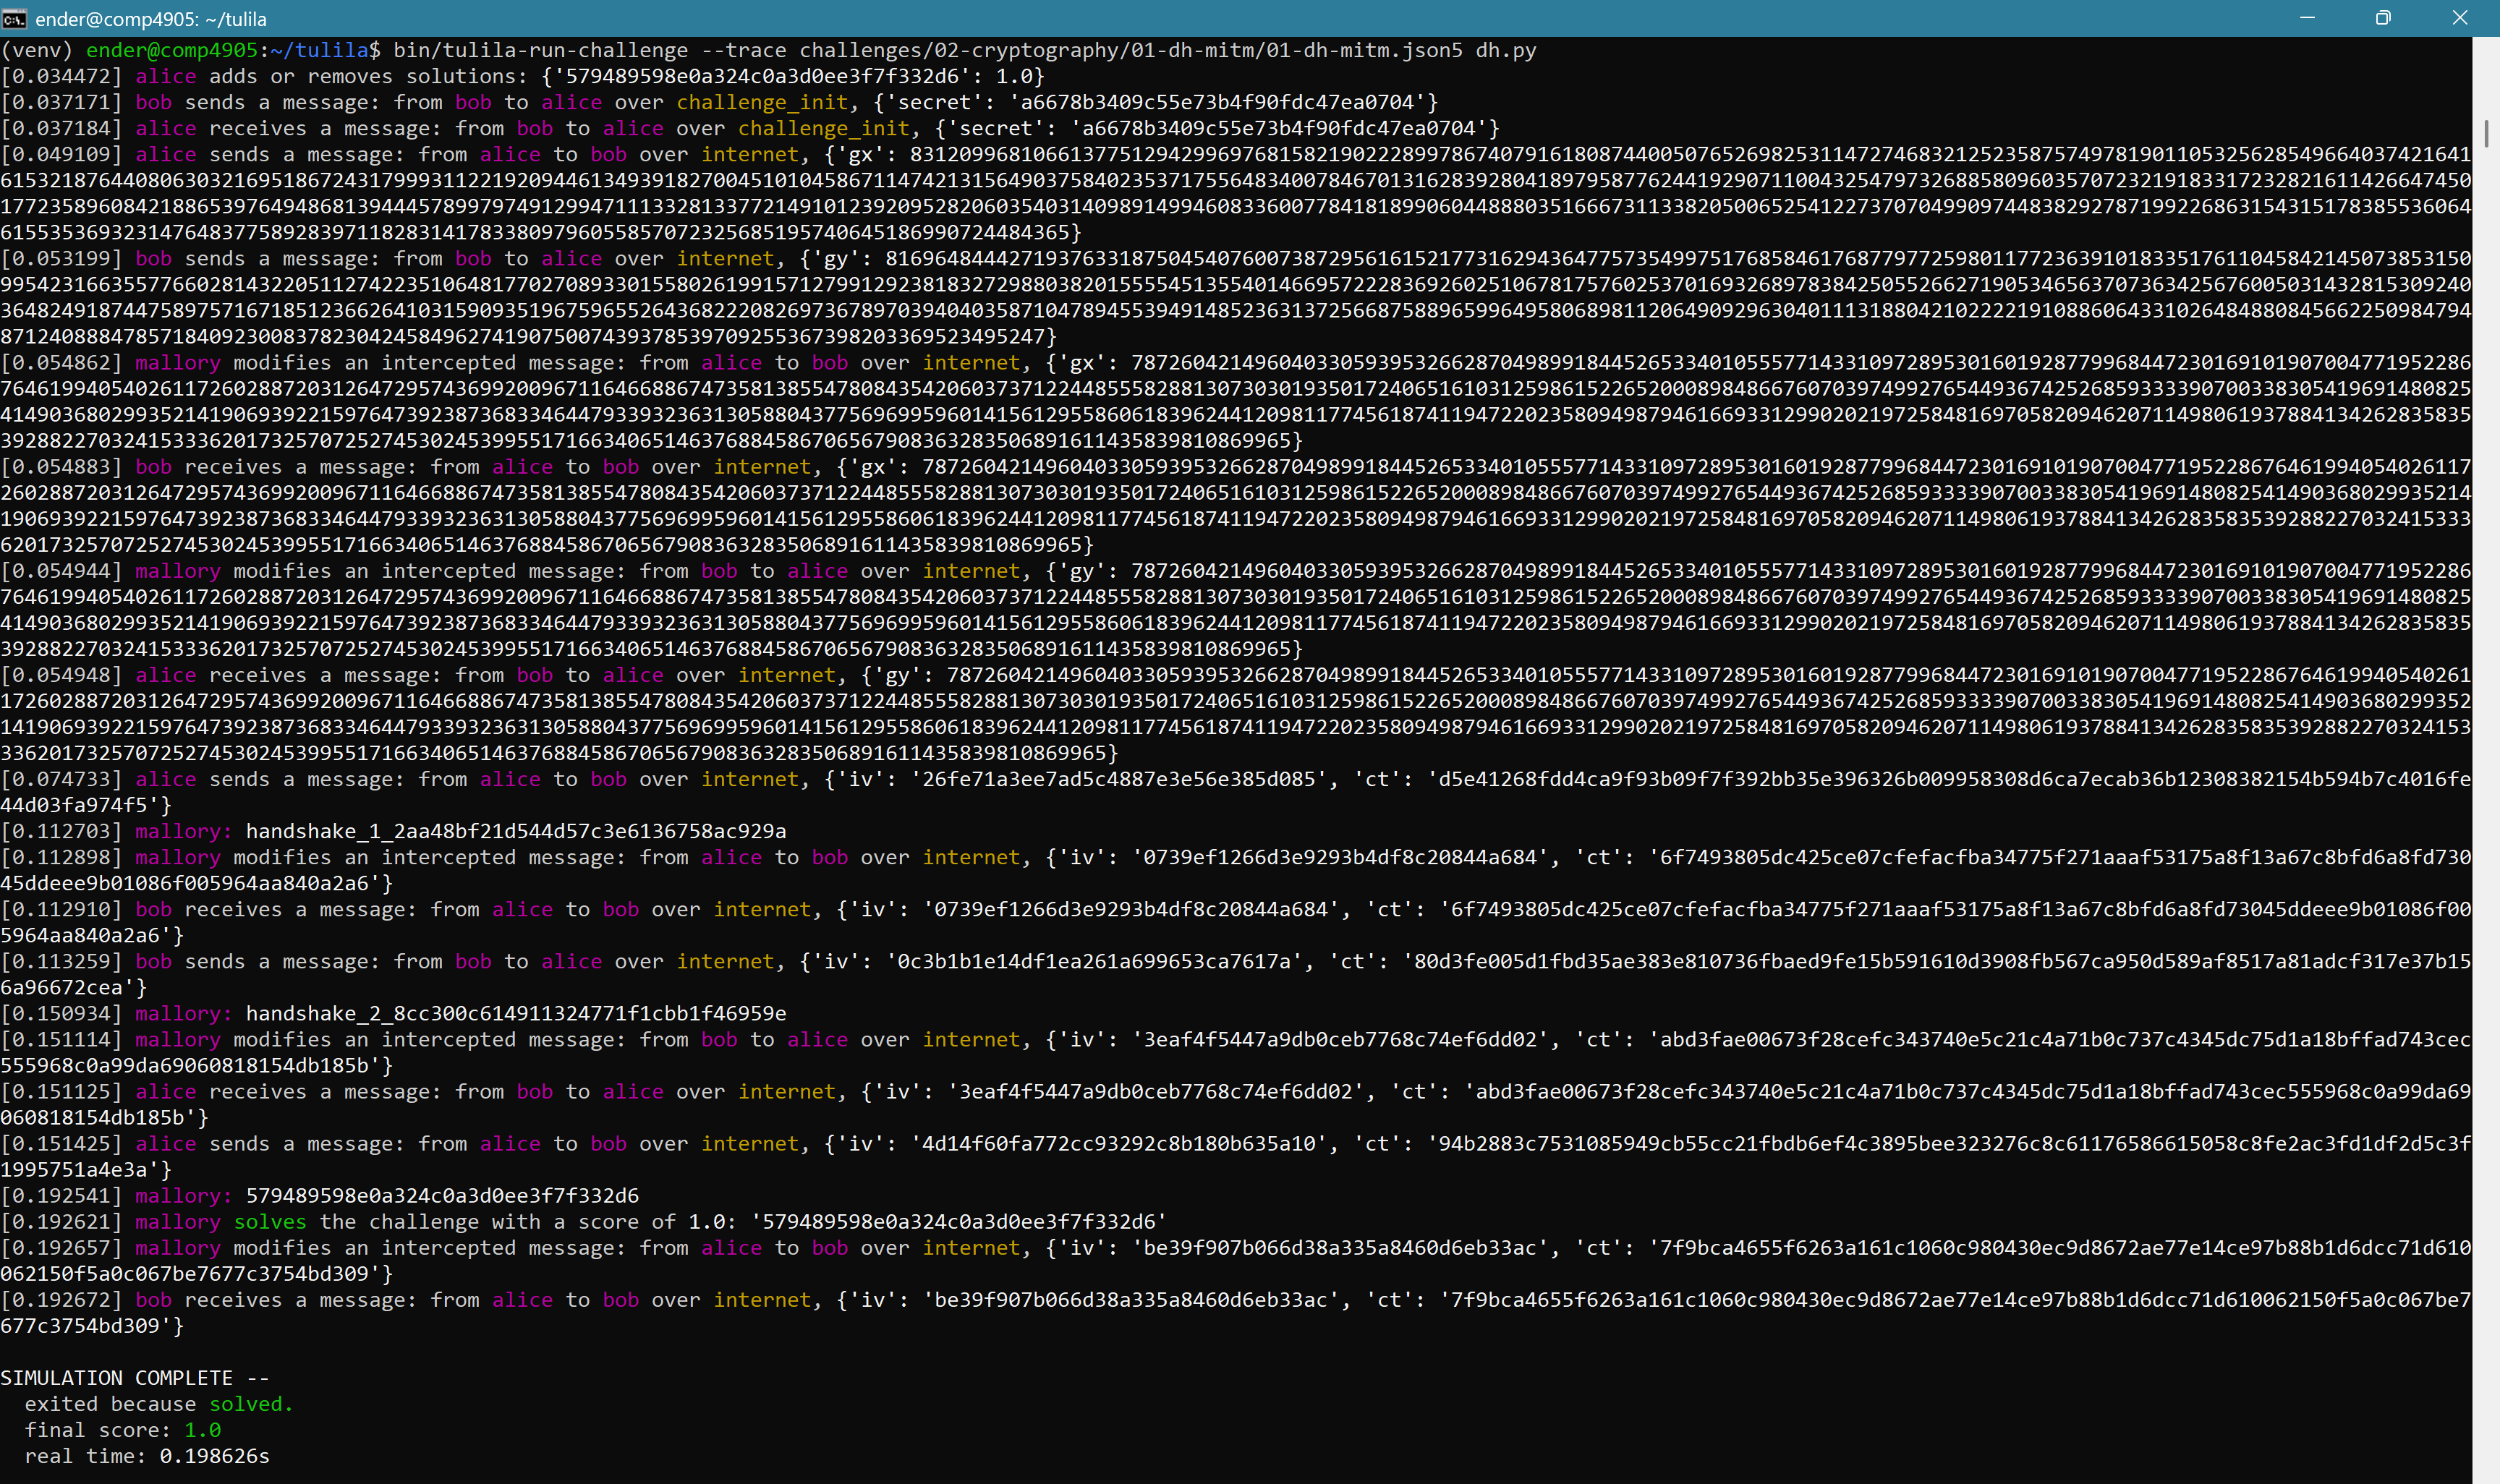
\includegraphics[width=\linewidth]{tulila-run-challenge}
  \caption{Sample run of \texttt{tulila-run-challenge}. The result section is slightly cut off---it is missing the line with the approximate CPU time.}
  \label{fig:tulila-run-challenge}
\end{figure}

\subsubsection{Tulila APIs}

Most of the Tulila APIs available to agents are covered in the tutorial series of challenges included with Tulila. Those that aren't can generally be learned by example from reading the included challenges. However, the included challenges do not include examples of setting up multiple solutions or finishing the challenge with partial credit (i.e., a score such that $0 < \text{score} < 1$). For your convenience, documentation for the entire API available to agents is included below; feel free to use any of this when developing your challenges.

\begin{small}
\begin{minted}{python}
def send(message_or_data, recipient=None, network="*", sender=None):
    """Send a message to another agent (or modify an intercepted message).
    
    The default network of "*" will be interpreted by the simulator code as "all
    networks I share with the recipient" for a non-broadcast recipient.
    
    You may broadcast to all recipients with "*", either on a given network
    or all networks (again with "*").
    """
    ...

def receive(*, timeout=-1):
    """Receive a message from another agent.
    
    The message will not necessarily be addressed to you, if you are
    a monitor or interceptor on a network.
    """
    ...

def drop():
    """Drop an intercepted message (the least recent such message that has not been handled).
    
    This is not meaningful for agents who are not interceptors on any network."""
    ...

def solve(s):
    """Try to solve the challenge with the given solution string."""
   ...

def set_solutions(solutions):
    """Modify the set of solution strings that will be accepted for this challenge run.
    
    Agents must have permission to do this.
    
    The solutions parameter should be a mapping between solution strings and scores
    between 0 and 1; a score of 0 will be interpreted as removing the string as a
    solution if it is so registered.
    """
    ...

def set_solution(s, score=1):
    """Add a solution string that will be accepted for this challenge run with the specified score.
    
    Agents must have permission to do this.
    """
    ...

def remove_solutions(solutions):
    """Remove a set of solution strings from this challenge run.
    
    Agents must have permission to do this.
    """
    ...

def remove_solution(s):
    """Remove a solution string from this challenge run.
    
    Agents must have permission to do this.
    """
    ...

def mark_solved(score=1):
    """Directly mark this challenge as solved with the specified score.
    
    Agents must have permission to do this."""
    ...
\end{minted}
\end{small}


\section{Design \& Implementation}

This section is a high-level overview of the design and implementation of Tulila, with a focus on the internal structure of Tulila and the ways in which it solves problems. It \textit{is not} the primary source for this information---that would be the source code of Tulila itself. This code is thoroughly documented and commented and is the definitive source of information on both \textit{how} Tulila was implemented and \textit{why} it was implemented that way. The section serves as a high-level ``map of the terrain'', and you are highly encouraged to consult the source code if you want more information on a particular part.

At the absolute highest level, Tulila is server software implemented in Python, except for the client component that runs in the user's browser, which is built in HTML, CSS, and JavaScript. A small amount of JavaScript implementing \href{https://wiki.debian.org/PolicyKit}{PolicyKit} rules is also included in the install script.
 
\sepfootnotecontent{module-or-package}{Technically, two packages and a module; in Python packaging parlance, a ``module'' is a file whereas a ``package'' is a directory. This distinction is not useful for the purposes of this document, so I will refer to all three as modules.}

Going into a bit more detail, Tulila is divided into three modules\sepfootnote{module-or-package}: \texttt{venvcache}, \texttt{tulila}, and \texttt{tulila\_server}. \texttt{tulila\_server} depends on \texttt{tulila} and \texttt{venvcache}, \texttt{tulila} depends on \texttt{venvcache}, and \texttt{venvcache} has no dependencies that I wrote. Each module will be discussed in turn, starting with \texttt{venvcache}.

Tulila must accept submissions of arbitrary Python code and execute them on the server. If you are security-minded, alarm bells \emoji{police-car-light} are going off in your head already---and indeed, this is difficult to do securely. By ``securely`` I mean that the system that executes arbitrary Python code must preserve the \textit{confidentiality} and \textit{integrity} of other data on the server---in short, submissions must not be allowed to \textit{read} or \textit{write} resources unless required for their normal operation. But this alone is insufficient. \textit{Availability} must also be maintained: a single submission must not be allowed to use up so many resources (CPU, RAM, disk, etc.) that it impairs the ability of other users to use the system. Careful design throughout Tulila was required to solve these problems (especially maintaining availability---any time Tulila does anything for an agent or a user, I must first think: ``how can I stop this from being abused?''). Designing to maintain these security properties will be a common theme throughout this section.

\subsection{\texorpdfstring{The \texttt{venvcache} Module}{The venvcache Module}}

The \texttt{venvcache} module is responsible for creating and caching virtual environments that each contain a specified set of dependencies. If you're not familiar with Python, you can think of a virtual environment as basically ``the folder with the dependencies for a certain program or script'', though this is a slight oversimplification.

Tulila allows challenge authors to specify dependencies that will be available to an agent in the challenge definition file. This is a requirement for many use cases---for example, the Diffie-Hellman Machine-in-the-Middle challenge included with Tulila requires the solution to \textit{use} AES (the Advanced Encryption Standard), but \textit{implementing} it is both rather complex and not an intended part of the challenge. Thus, Tulila allows challenge authors to make any package from \href{https://pypi.org/}{the Python} \href{https://pypi.org/}{Package Index} (PyPI) available to an agent's code just by adding it to the challenge definition file. \texttt{venvcache} is what makes that possible behind the scenes.

The best way to understand this module is by its public API. This API is consumable either by creating a \texttt{VenvCache} object \textit{or} by using a per-process singleton \texttt{VenvCache} object whose methods are exported from the module itself; this follows a pattern also seen in Python's built-in \texttt{random} module. The key information distinguishing different \texttt{VenvCache} instances is the directory in which the virtual environment cache is stored; the default for the per-process singleton is \texttt{\textasciitilde{}/.venvcache}. The public API is:

\begin{enumerate}
  \item \texttt{set\_directory(path)}, set the directory of the virtual environment cache.
  \item \texttt{async setup(deps)}, create a virtual environment that satisfies the given set of requirements or use a cached one, then return the path to the Python interpreter in it. \texttt{deps} is a list of \href{https://pip.pypa.io/en/stable/reference/requirement-specifiers/}{requirement specifiers}; this may optionally specify versions for each dependency.
  \item \texttt{interpreter(deps)}, if there exists a cached virtual environment that matches the given set of requirements, return the path to the Python interpreter in it.
  \item \texttt{mark\_venv\_used(deps)}, an alias for \texttt{interpreter}.
  \item \texttt{includes(deps)}, return a boolean value indicating if there exists a cached virtual environment that matches the given set of requirements.
  \item \texttt{clean()}, delete all unused virtual environments from the cache. A virtual environment is considered used if and only if it has been referenced by \texttt{setup}, \texttt{interpreter}, or \texttt{mark\_venv\_used} since the \texttt{VenvCache} object was created.
\end{enumerate}

To be clear, it is desirable to cache virtual environments because they take a long time to create. This is both because the virtual environment creation routines built in to Python are oddly slow and because it takes time to download and install the transitive closure of the specified dependencies.

Each virtual environment is created and cached in a directory named by (a) sorting the dependency requirement specifiers lexicographically; (b) joining them with the newline character; and (c) hashing them with SHA256 and hex-encoding the digest. This is guaranteed to always produce a value that is both filesystem-safe and unique for a given set of requirement specifiers (if not necessarily unique for a given set of dependency versions actually fetched from PyPI; consider, e.g., requirement specifiers ``\texttt{foo==3}'' and ``\texttt{foo>2,foo<4}'').

Some additional considerations handled by \texttt{venvcache} include correctly handling errors in virtual environment creation, tracking which virtual environments have been used, and abstracting away differences between platforms. These aspects are not notable enough to be fully documented here but, as always, are documented in the source code itself.

\texttt{venvcache} is self-contained, relatively small, and provides a broadly useful service. As such, I designed and implemented it to be completely separate from the rest of Tulila. It is a standalone module and can be re-used by any other project that finds its functionality useful.


\subsection{\texorpdfstring{The \texttt{tulila} Module}{The tulila Module}}

The \texttt{tulila} module implements the core challenge and simulation functionality of Tulila including the object model, the agent sandbox, and the simulator. It does not implement the Web interface or administrative tools---those live in \texttt{tulila\_server}. I will start this section by discussing the public API of \texttt{tulila}; this will be followed with more information on particularly interesting facets of the internal implementation.

\subsubsection{Public API \& Object Model}

\texttt{tulila}'s public API was designed with separation of concerns in mind; essentially, the goal was to expose only what is absolutely necessary for the API consumer to ``know'' and keep as much complexity as possible hidden behind the abstraction barrier. From this I derived the following requirements:

\begin{enumerate}
  \item It should be easy to describe agents, networks, and challenges in terms of the public API. There should be a type representing each of these concepts.
  \item Internal simulation concepts should be hidden as much as possible. There should be a function that accepts a submission's code and returns (a coroutine returning) a result object (this hides the implementation details of the simulator---all the calling code knows is ``given a submission, I can get a result'').
  \item This module is not concerned with users. Simulation results generated by this module are not associated with any particular user---that is the responsibility of the calling code.
  \item Similarly, this module is not concerned with the fiddly details of running multiple simulations concurrently. It should provide enough tools to allow higher level code to do this, but need not concern itself with details like how many can run at once.
\end{enumerate}

These requirements also keep the parts of Tulila that could potentially be re-used by other projects separate from the ones that are more specific to my particular use case. Overall, I am quite happy with the API that I ended up with.

To start understanding \texttt{tulila}'s public API, first look at the object model in \cref{fig:tulila-class-diagram}. This is easily the most important part of the public API. These types represent agents, networks, and challenges within Tulila. They are immutable after creation and contain fields for all of the attributes that are used by Tulila's simulator, along with a ``\texttt{metadata}'' field. This field contains arbitrary metadata that was present in the JSON5 challenge definition file, but is not used by the simulation (lots of stuff used by \texttt{tulila\_server} is ultimately loaded through this mechanism).

That is a good segue to another responsibility of \texttt{tulila}: loading challenges from JSON5 files. \texttt{tulila} exposes the \texttt{load\_challenge} and \texttt{load\_challenges} functions for this. Challenges, and their associated objects, can be created using these functions or by manually invoking the constructors (the constructors are eventually invoked either way). The constructors perform extensive validation, e.g., rejecting the creation of a \texttt{Challenge} containing a \texttt{Network} that names a member not in the challenge's collection of \texttt{Agent}s. Agents and networks do tend to be referenced by name---this is because constructing mutually referential immutable objects isn't really possible and to better reflect the structure of JSON5 challenge definition files. Maps associating names with the actual objects are available after the challenge and its associated objects are created via a \href{https://docs.python.org/3/library/functools.html#functools.cached_property}{\texttt{@cached\_property}}.

\begin{figure}[ht]
  \centering
  \subsubfigintoc{Class diagram of the \texorpdfstring{\texttt{tulila}}{tulila} module}
  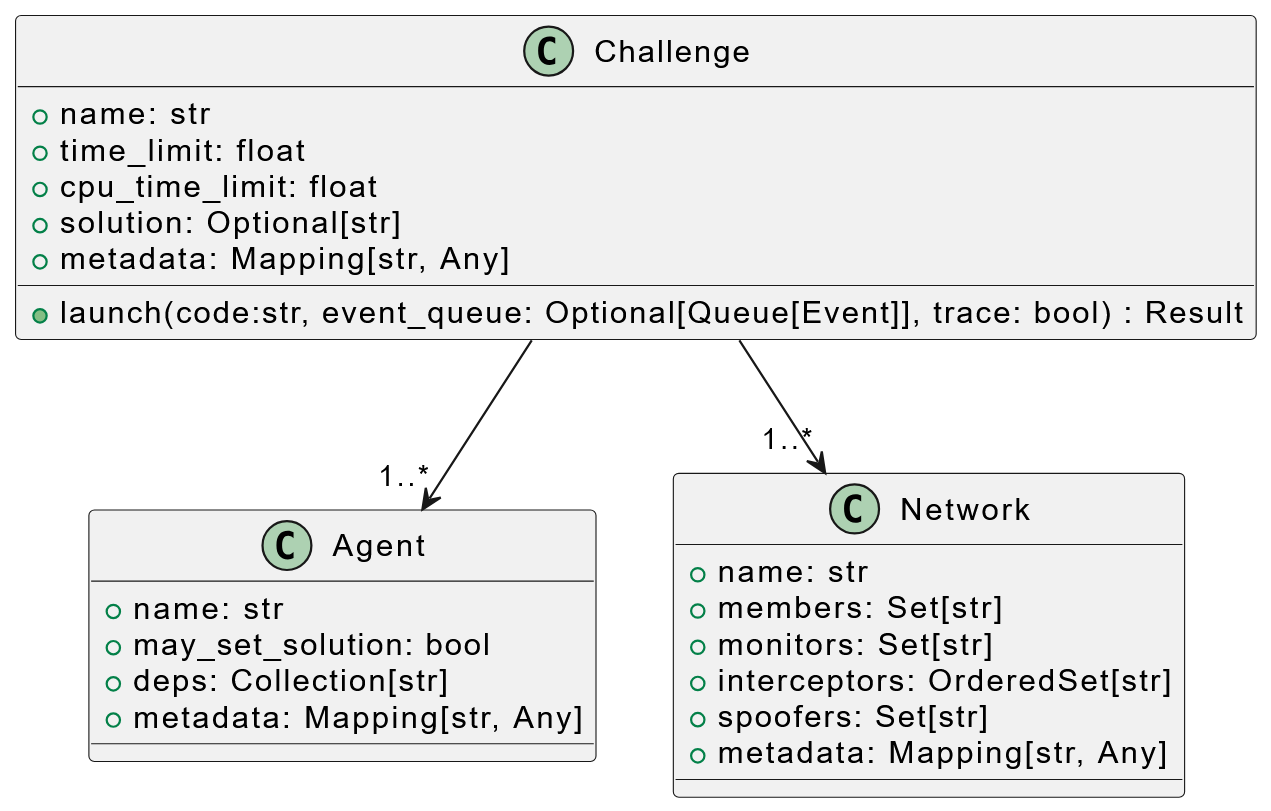
\includegraphics[width=\linewidth]{tulila-class-diagram}
  \caption{A simplified class diagram of the \texttt{tulila} module, focusing on the relationships between the most important classes. Simple record types such as \texttt{Result} are excluded.}
  \label{fig:tulila-class-diagram}
\end{figure}

The other important function in the public API is the asynchronous \texttt{launch} method on the \texttt{Challenge} type. This method implements ``submitting to a challenge'': it takes as a parameter the code to use as the solution and returns the result. The result is an instance of a record type containing the score, exit reason, time, and approximate CPU time. Simulations run asynchronously via standard \texttt{asyncio} primitives; as such, calling code can, e.g., run multiple simulations concurrently (using something like \texttt{asyncio.gather}).

To aid in debugging, the \texttt{launch} method also takes an optional \texttt{event\_queue} parameter: an \texttt{asyncio} queue to which events generated during the simulation will be pushed. These can be received by calling code while the simulation is still running by careful use of \texttt{asyncio} APIs (most simply, \texttt{wait}). These events are intended for debugging only---the only thing calling code can do is display them in some way, as there is no way to manipulate the simulation state via these events. Exposing events like this lets \texttt{tulila} be frontend agnostic, i.e., multiple frontends for submitting to a challenge, viewing the result, and debugging your submission can be implemented. And, indeed, two such frontends \textit{were} implemented: \texttt{tulila\_server} (\cref{section:the-tulila-server-module}) and \texttt{tulila-run-challenge} (\cref{section:testing-challenges}).

\subsubsection{Agent Sandbox}

As discussed earlier, it is important to maintain the confidentiality and integrity of other data stored on the server where submissions are to be run. Thus, agent code must be sandboxed. At the very highest level, a sandbox can be based on an \textit{allowlist} (default-deny, allow what is on the list) or a \textit{denylist} (default-allow, deny what is on the list). These options have \textit{vastly} different security properties: a missing rule on a denylisting sandbox is a breach waiting to happen whereas a missing rule on an allowlisting sandbox merely breaks functionality. Thus, I chose to go with an allowlisting sandbox.

The tool I used to implement the agent sandbox is Justine Tunney's \href{https://justine.lol/pledge/}{\texttt{pledge}} tool for Linux (itself inspired by the API of OpenBSD's \href{https://man.openbsd.org/pledge.2}{pledge syscall}). The remainder of this paragraph is information adapted from \texttt{pledge}'s documentation and source code. \texttt{pledge} uses two Linux kernel facilities to create a sandbox: \href{https://www.kernel.org/doc/html/v4.17/userspace-api/seccomp_filter.html}{SECCOMP BPF} and the \href{https://docs.kernel.org/security/landlock.html}{Landlock LSM}. SECCOMP BPF allows a process to load small programs expressed in BPF bytecode into the kernel to filter syscalls; these programs will be run whenever the process or a child process executes a syscall and may choose to deny the syscall. Once installed, these filters cannot be removed. New filters may be installed but this can only further restrict the process (as all installed filters must permit the syscall for it to be allowed). BPF is a simple bytecode format that is used extensively for hooks in the Linux kernel because of some interesting properties---most notably, it is possible to prove a BPF program will terminate (regardless of input). SECCOMP BPF filters are very powerful, but they have some limitations that stem from their inability to inspect values that are not directly passed in to the syscall (they make decisions with very little ``context''). As such, SECCOMP BPF alone cannot restrict filesystem access by path (that would require, at minimum, the ability to follow pointers). Landlock LSM fills this gap: \texttt{pledge} uses this API to restrict the process and subprocesses to a specified set of files, directories, and permissions (i.e., read, write, execute). Some ancillary functions of \texttt{pledge} are implemented in terms of other APIs as well.

\texttt{pledge} is very simple to use; my invocation of \texttt{pledge} is as follows (with comments removed as I discuss it in the prose):

\begin{minted}{python}
proc = await create_subprocess_exec(
    "pledge", "-n", "-q", "-M", str(VM_LIMIT),
    
    "-p", "stdio rpath tty prot_exec",
    "-v", _AGENT_LOADER_PATH,
    "-v", dirname(dirname(interpreter)),
    
    interpreter, _AGENT_LOADER_PATH,
    env=_AGENT_ENV,
    stdin=PIPE, stdout=PIPE, stderr=PIPE
)
\end{minted}

The options I use are:
\begin{enumerate}
  \item ``\texttt{-v}'' specifies paths that the agent may access (read-only; \textit{no} paths are opened to writing and I don't recall the syntax for doing so). The agent is allowed to access the agent loader script (see \cref{section:simulator}) and its own virtual environment.
  \item ``\texttt{-p}'' specifies what the agent is allowed to do, using categories built in to \texttt{pledge}. I specify ``\texttt{stdio rpath tty prot\_exec}''. Specifying some of these implicitly allows access to other paths not specified with ``\texttt{-v}''; this is mostly stuff like \texttt{/dev/null}, \texttt{/dev/urandom}, etc, but notably does include all of \texttt{/lib}. (This is unfortunate, but it is impractical to enumerate exactly which shared objects are required, especially as agents may be given access to anything from PyPI by the challenge author.)
  \begin{itemize}[$\circ$]
    \item ``\texttt{stdio}'' grants access to the process's own standard input, output, and error.
    \item ``\texttt{rpath}'' allows the process to open files for reading if such access is granted by a ``\texttt{-v}''. (Note here that the absence of ``\texttt{wpath}'' prevents the agent from opening files for writing \textit{even if such access was granted by a ``\texttt{-v}''}. This is an example of defense-in-depth.)
    \item ``\texttt{tty}'' grants access to terminal IOCTLs. Agents do not, in general, run under a terminal, but I observed that this was required to cut down on line-spam generated by Python at startup. If an agent \textit{is} run under a terminal, this does let them mess it up (e.g., by disabling echo of input); this annoyance can be fixed by restarting the terminal and does not constitute a sandbox breach.
    \item ``\texttt{prot\_exec}'' allows the agent to allocate new executable memory. This is required as libraries from PyPI sometimes want to load shared objects.
  \end{itemize}
  \item ``\texttt{-n}'' runs the process with maximum ``niceness'', only using idle CPU cycles. This prevents a CPU-heavy agent from hogging resources and impairing the ability of Tulila or other services to function.
  \item ``\texttt{-M}'' limits the amount of RAM the process may use. Similar to ``\texttt{-n}'', this stops a malicious or broken agent from using more than its share of a shared resource.
  \item ``\texttt{-q}'' tells \texttt{pledge} to be quiet, i.e., not to log violations to standard error.
\end{enumerate}

I chose \texttt{pledge} as my sandboxing solution because it is lightweight and simple. Having completed Tulila, I am happy with that choice. \texttt{pledge} was extremely easy to use and starts \textit{very} fast---it takes on the order of tens of milliseconds to launch an agent and that includes time spent initializing the Python interpreter in the agent process. It goes without saying that this is much faster than any virtualization-based sandbox. \texttt{pledge} uses the same kernel as the host, greatly reducing overhead.

\subsubsection{Simulator}
\label{section:simulator}

The design of the sandbox---completed early in Tulila's development---influenced the design of the simulator. The object that \texttt{pledge} sandboxes is a \textit{process}; therefore, agent code must run in its own process. The natural way of communicating with agents, then, is via standard in and out---so that is what the simulator does.

A rough sketch of the lifecycle of a simulation follows.

\begin{enumerate}
  \item The simulator launches all of the agents in their own processes. \texttt{pledge} is used to sandbox a Python interpreter; this interpreter is not passed the agent code directly but instead runs the ``Agent Loader.'' This is a short Python program that (a) accepts the agent code over standard in; (b) sets up the environment the agent runs in, providing functions like \texttt{send} and \texttt{receive} to allow it to interact with the simulation; and (c) runs the agent code.
  \item The simulator waits for an agent to print a line to standard output or error.
  \begin{itemize}[$\circ$]
    \item Lines printed to standard error become debug prints in the event queue.
    \item Lines printed to standard output are interpreted as requests to the simulator. These are encoded in JSON, and in response the simulator will perform the requested action (e.g., copying a sent message to another agent's standard in for it to receive). Agents can only communicate by requesting that the simulator forward a sent message to another agent; there is no way for them to communicate directly. Some requests will be denied by the simulator unless the agent has permission (e.g., setting the solution).
    \item Lines that exceed a configurable line length limit will be discarded without being processed. This prevents a single agent from tying up an undue amount of resources and also allows a limit on the number of lines to meaningfully limit the total size of a log; this property is used by \texttt{tulila\_server}.
  \end{itemize}
  \item The simulation ends when any agent process exits, when the challenge is solved, or when a time limit (CPU or real) is exceeded.
\end{enumerate}

In my project proposal, one of my stretch goals was to design and implement a mechanism that provided submissions with equal access to CPU time regardless of the current load on the server. This was inspired by my experience in COMP 2402 Abstract Data Types and Algorithms where student code, judged on speed, would run slower if the server was under load (perhaps from many submissions). While I do appreciate the ``cosmic justice'' of rewarding those that start their assignments early, this isn't a particularly fair system. To give all submissions a fair shake, the Tulila simulator measures their total CPU time and allows challenge authors to set a CPU time limit in addition to a real time limit. This can be used to ensure that all submissions are given the, e.g., 0.25 seconds of CPU time required to solve the challenge regardless if that takes 0.25 seconds (under light load) or 5 seconds (under heavy load).

The CPU time of a submission is defined as the total user and kernel CPU time of all the agent processes in that submission's simulation. This is better than just measuring the CPU time of the agent submitted by the user as that approach does not adequately capture situations where a provided agent does work on behalf of the submitted agent (e.g., in a padding oracle challenge). This time is measured by regularly sampling \texttt{/proc/<pid>/stat} for all agent processes that make up the simulation.

\subsubsection{Quality Assurance}

Throughout the course of this project, I took many steps to ensure the software I was building worked as intended with minimal errant behavior (``bugs''). I will not discuss all the techniques I used as they do not all have enough insight to justify the space. However, I would like to highlight the two most significant techniques I used and the lessons learned from them: static typing and coverage testing.

Python is a dynamically typed language; that is, the type of the value stored in a variable is not known until runtime. The alternative is static typing, where the types of variables (including function arguments, fields, etc.) are known before the code is run. Static typing makes it possible to catch many types of bugs early---a simple example is calling \texttt{math.floor("3")}. Statically-typed languages will refuse to compile this as \texttt{math.floor} expects some kind of number type, which \texttt{"3"} is not---it's a string! Clearly, the programmer forgot a call to \texttt{int} (or something). Static typing can help catch many of these kinds of errors (generally much more complex than the trivial example above---consider, e.g., setting a variable 80 lines above where it is used), making it an invaluable tool to improve the correctness of a program.

\sepfootnotecontent{which-pep}{The syntax for annotations was added in \href{https://peps.python.org/pep-3107/}{PEP 3107}, which predated PEP 484 but did not include semantics for type-checking.}

Python added \textit{optional} static typing in a series of PEPs (Python Enhancement Proposals) starting with \href{https://peps.python.org/pep-0484/}{PEP 484}\sepfootnote{which-pep}. These don't change how the language is evaluated at all; rather, they provide space in the syntax for type information and a standard way for type-checking tools to use this information in a separate type-checking pass that may be performed before the program is run. One such type-checking tool is \href{https://mypy-lang.org/}{\texttt{mypy}}. I decided to type-check all of Tulila's Python code with \texttt{mypy} in order to find and fix bugs and improve its correctness. This required adding and maintaining type annotations on every function and field, as well as some variables for which the type could not be inferred.

Overall, I'm happy with my decision to type-check Tulila with \texttt{mypy}---I definitely found some bugs with it that I may not have caught otherwise. Certainly it's faster and easier to detect bugs with \texttt{mypy} before even running the code than with tests far down the line. \texttt{mypy} also offered me the ability to ``fearlessly refactor''---I could easily change the parameters expected by a function and \textit{know} with certainty that I updated all the callsites. I used this many times throughout the course of development as I was building and experimenting with different API designs.

With that said, \texttt{mypy} has some limitations. First off, it obviously cannot detect every type of bug. But beyond that---idiomatic Python uses lots of duck typing, and duck typing is certainly a tool I employ quite a bit. Expressing this in \texttt{mypy} and getting everything to type-check correctly was frustrating at times, especially due to the lack of an intersection type. For example, expressing a type that's ``like an \texttt{asyncio} \texttt{Process}, but \texttt{stdout}, \texttt{stderr}, and \texttt{stdin} are definitely not \texttt{None}'' is quite difficult to do without an intersection type---I needed 29 lines to express this. Defining the \texttt{OrderedSet} type was a chore as well, in part due to \texttt{mypy}'s often arbitrary distinction between abstract base classes and protocols. Working around poor type annotations in third-party libraries was another source of frustration. Overall, I would describe \texttt{mypy} as a useful tool, but it still has room to grow.

Another technique I used was coverage testing. This is a form of testing in which you run a monitoring tool that makes sure your tests hit every line and branch of the code that is being tested. This is thorough, but it is time-consuming to write so many tests. I ran coverage testing on a part of Tulila for which correctness was imperative: the simulator (see \cref{fig:coverage-testing}). This is the code that evaluates user submissions and any correctness issue here has the potential to be \textit{very} frustrating for users. This code also has many complicated and subtle behaviors and has to handle the interactions between many different features---edge cases abound! (This is in contrast to, e.g., the code that loads challenges from JSON5 challenge definition files: if that code breaks, it impacts only the challenge author and the breakage will be early and obvious.)

\begin{figure}[ht]
  \centering
  \subsubfigintoc{Coverage testing of Tulila's simulator}
  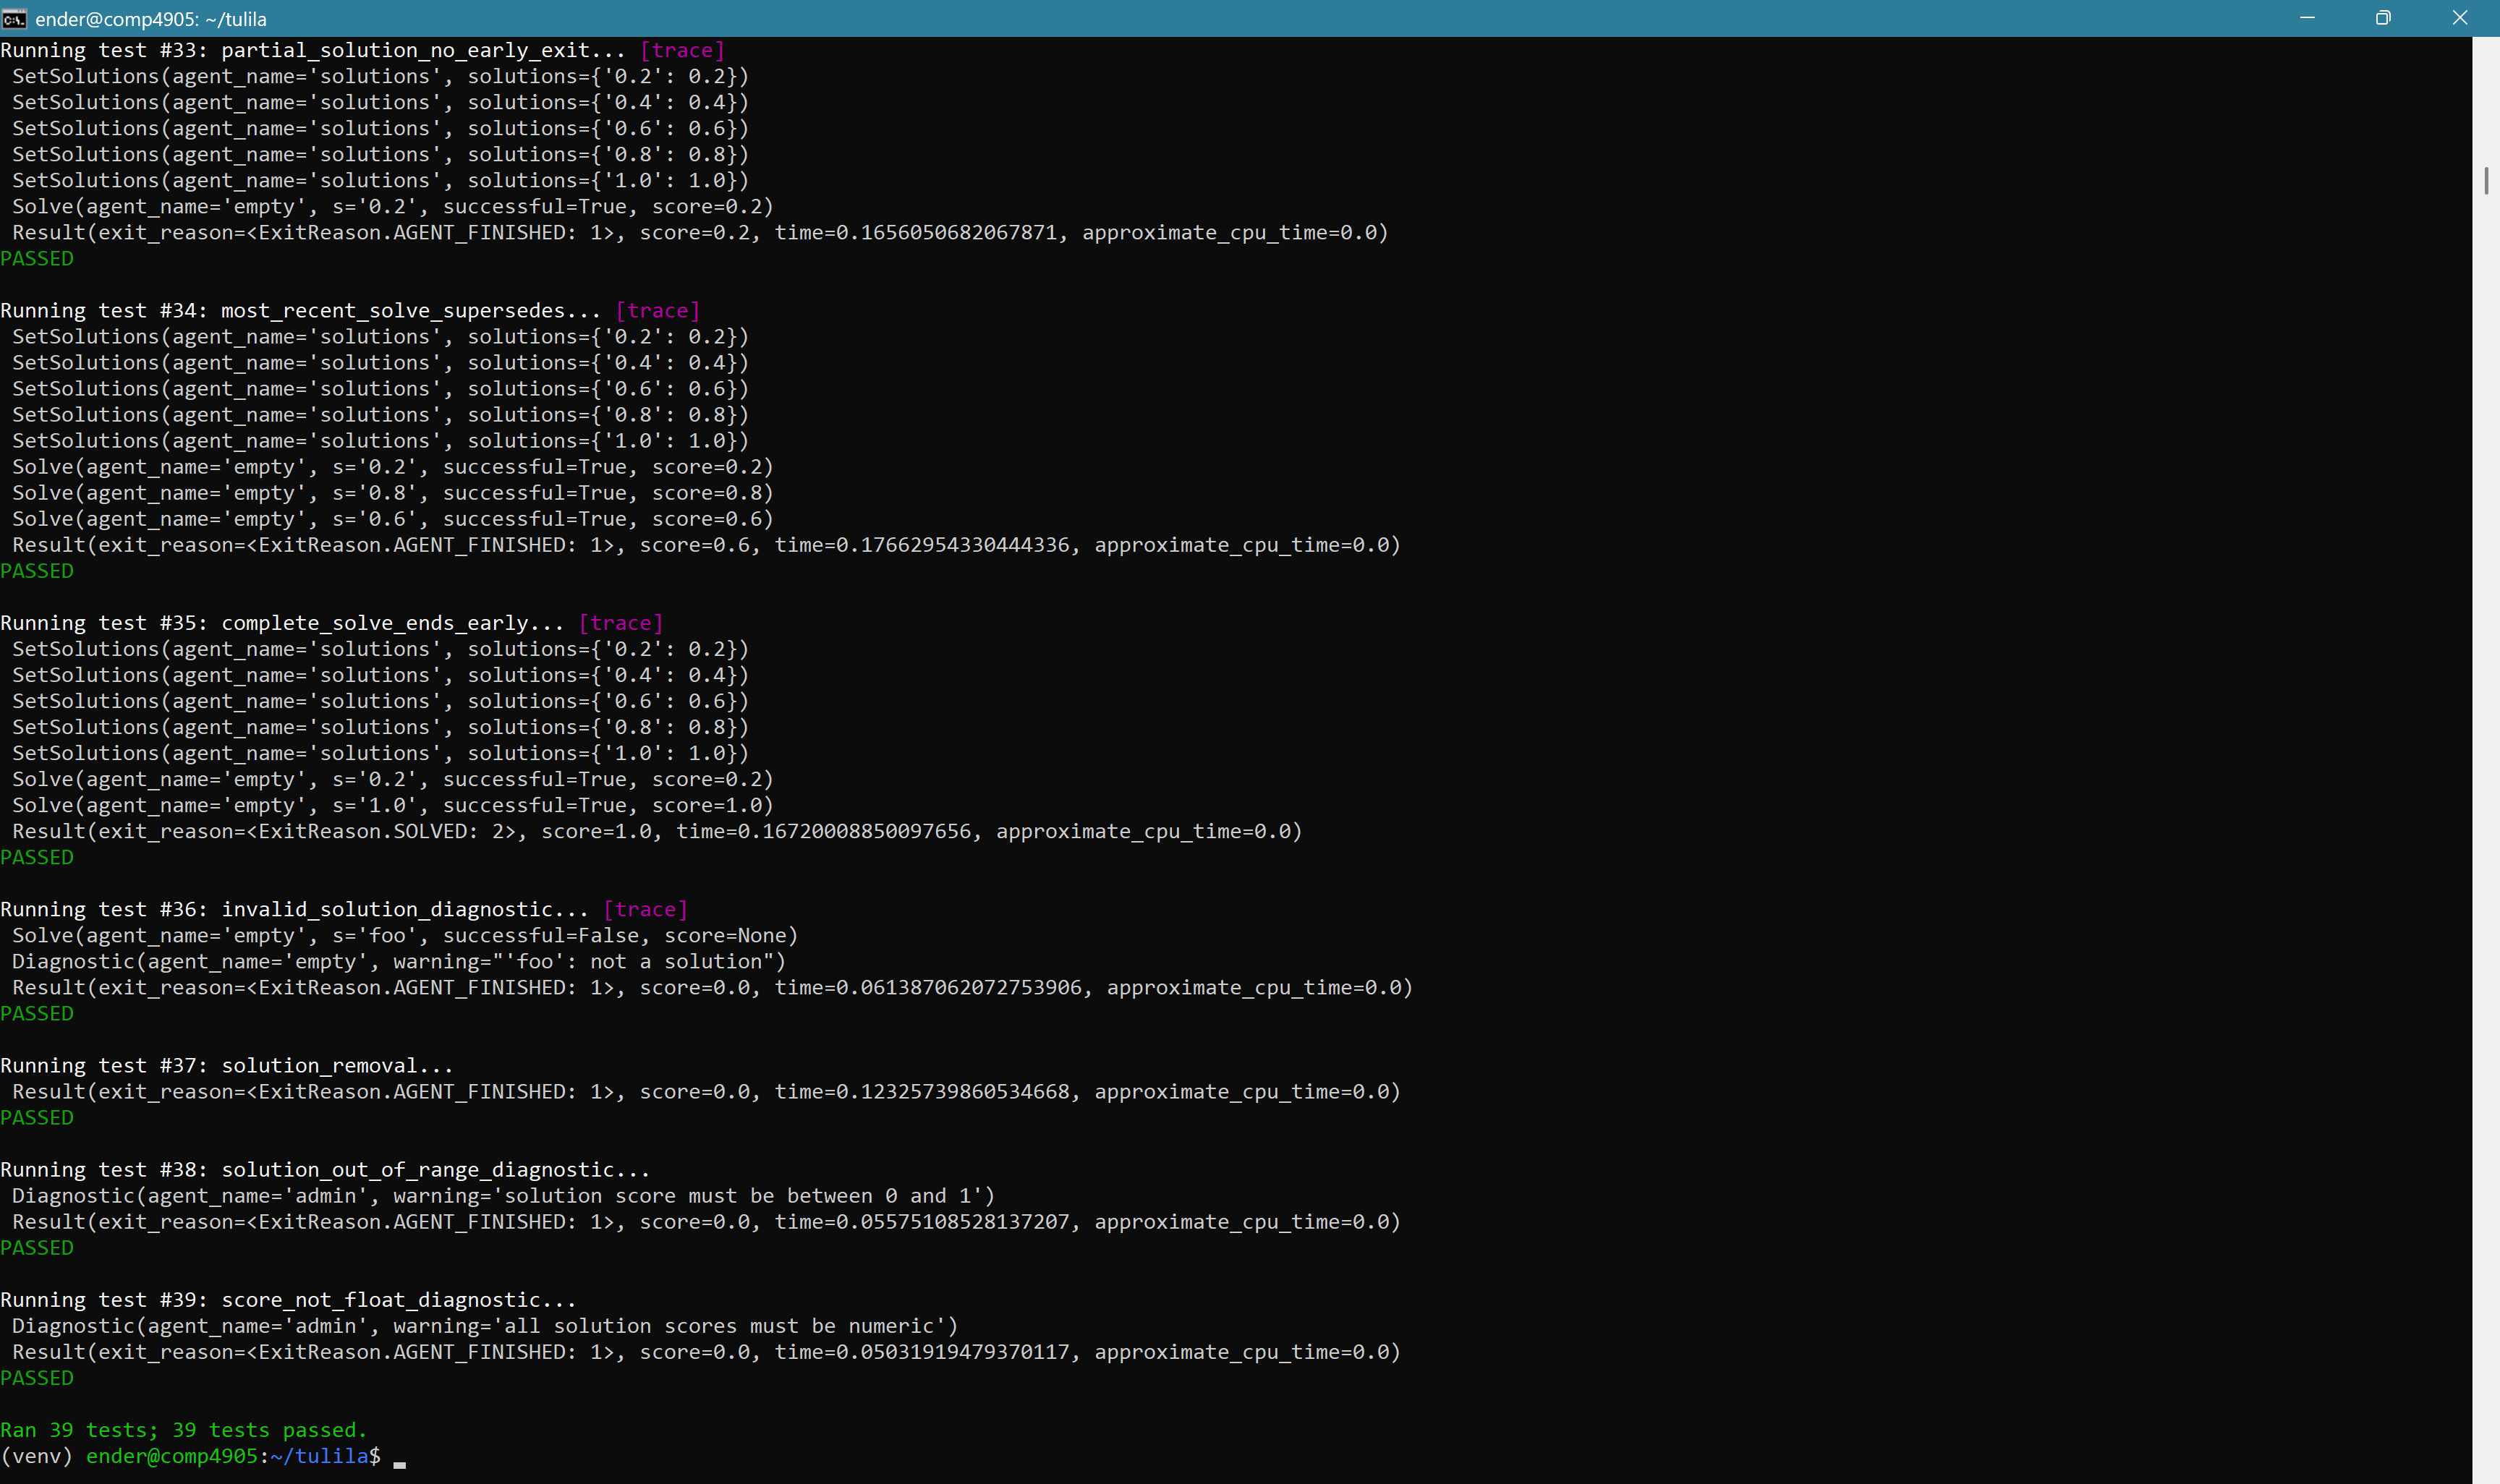
\includegraphics[width=\linewidth]{coverage-testing}
  \caption{Coverage testing of Tulila's simulator. The end of a test run is pictured, showing that 39/39 tests passed.}
  \label{fig:coverage-testing}
\end{figure}

I wrote 39 tests for the simulator (in \texttt{dev-scripts/simulator-cov.py}); together, these exercise almost every line and branch of the simulator code. In the process of writing these tests, I discovered 3 bugs, so it was certainly a worthwhile endeavor. Unfortunately, not quite \textit{every} line of the simulator code is hit by the coverage tests: a few lines that required either winning a race condition or generating an \textit{unexpected} exception to hit were excluded. Overall, I'm quite happy with my decision to coverage test the simulator; it gave me some much-needed confidence that the code I was building on was correct.


\subsection{The \texorpdfstring{\texttt{tulila\_server}}{tulila\_server} Module}
\label{section:the-tulila-server-module}

\texttt{tulila\_server} implements the user interface of Tulila (shown in \cref{fig:tulila-ui}), for both users and administrators. It allows remote users to log in, submit to challenges, and view their previous submissions and scores. For administrators, \texttt{tulila\_server} provides the implementation of the tools for creating users and exporting scores (\texttt{tulila-reset} and \texttt{tulila-run-challenge} are standalone---they don't live in any module).

\texttt{tulila\_server} is an \texttt{aiohttp} Web application that persists data in SQLite using the SQLAlchemy ORM. HTML pages sent to clients are generated using the Jinja2 template engine and, for the most part, user interaction is handled through server-rendered responses. A small amount of client side JavaScript is used to support the submission editor and live viewing of debug events while a submission is running (via a WebSocket).

\begin{figure}[ht]
  \centering
  \subsubfigintoc{Tulila's user interface}
  
\includegraphics[width=\linewidth]{tulila-ui}
  \caption{Tulila's user interface. The challenge listing page is shown, displaying 10 challenges organized into 2 categories (``Tutorial'' and ``Cryptography''). The logged-in user has successfully completed 6 of the 7 tutorial challenges included with Tulila.}
  \label{fig:tulila-ui}
\end{figure}

Full credit for all third-party software libraries and content included with Tulila is in \cref{section:third-party-content}; however, I would like to make special mention here of two of the bigger pieces of third-party content in \texttt{tulila\_server}.

\begin{enumerate}
  \item The CSS styles used in \texttt{tulila\_server} are \textit{heavily} based on \href{https://watercss.kognise.dev/}{Water.css by Kognise} (released under the free and open source \href{https://github.com/kognise/water.css/blob/master/LICENSE.md}{MIT license}). I just made some light tweaks, mostly related to fonts, and added a small number of custom styles. No part of the \textit{functionality} of Tulila is implemented by Water.css, but it sure makes it look better! (A welcome addition, as my own sense of style is nonexistent.)
  \item The banner image, which can be seen in \cref{fig:tulila-ui}, was drawn by Adrien ``doggkidd'' Boileau under commission (i.e., I paid them). Thanks Adrien!
\end{enumerate}

With that out of the way, let's move on to discussing the internal structure of \texttt{tulila\_server}.

\subsubsection{Internal Structure}

\texttt{tulila\_server} is divided into 10 submodules. Most of these submodules implement a piece of functionality for the rest of \texttt{tulila\_server} to consume, following the principle of separation of concerns. A short description of each submodule follows. (Note that submodule names start with ``\texttt{\_}'', by convention, to indicate that they should not be imported from outside \texttt{tulila\_server}; i.e., they are not part of the public API).

\begin{enumerate}
  \item \texttt{\_authentication} implements user log-in and sessions. I chose to discuss this submodule first as it is a great example of how the API design of \texttt{tulila\_server} submodules encapsulates complexity. The API exported by \texttt{\_authentication} is only three functions:
  \begin{itemize}[$\circ$]
    \item \texttt{requires\_authentication}, a decorator that can be applied to a route handler to indicate that it should be restricted to logged-in users.
    \item \texttt{who}, given a request object return the associated user.
    \item \texttt{init\_authentication}, called once while Tulila is starting to make \texttt{who} and \\\texttt{requires\_authentication} work.
  \end{itemize}
  All of the complexity related to how users are authenticated, how sessions are stored, etc, is completely encapsulated---all API consumers have to do is indicate that a route should be gated behind login and that just happens, ``magically''. I will not be including the APIs of other submodules here, but I chose to do so for \texttt{\_authentication} as it's a good example of my philosophy of software design.
  \item \texttt{\_challenges} loads the registered (see \cref{section:adding-challenges}) challenge definition files and organizes challenge data in the way that is maximally convenient for the rest of \texttt{tulila\_server} to consume. It is also responsible for parsing the metadata fields used by Tulila's user interface and loading data from sidecar files (as appropriate). Challenge categories, which are not a concept in \texttt{tulila}'s ontology, are implemented here.
  \item \texttt{\_config} loads \texttt{tulila\_server}'s configuration from environment variables.
  \item \texttt{\_csrf\_protection} protects routes that modify server state from \href{https://owasp.org/www-community/attacks/csrf}{CSRF attacks}.
  \item \texttt{\_database} provides a convenient, object-oriented interface to Tulila's SQLite database (using SQLAlchemy).
  \item \texttt{\_egg} is intentionally undocumented---it implements a fun secret you must discover for yourself.
  \item \texttt{\_graphviz} creates pretty graphical representations of Tulila challenges, visualizing the agents, networks, and relationships between them. It also handles caching these graphical representations for later re-use. As the name implies, it uses \href{https://graphviz.org/}{Graphviz} internally for layout.
  \item \texttt{\_submissions} implements the submission manager: a rather complicated component of Tulila that is responsible for handling submissions from the moment they are submitted until the results are saved in the database, advancing them through their lifecycle when it is appropriate to do so. Much of this complexity, including the rules around running simulations concurrently, is intended to prevent a single user from using so many resources that it impairs the ability of other users to access the system (i.e., improving the \textit{availability} of Tulila).
  \item \texttt{\_routes} contains the HTTP route handlers of \texttt{tulila\_server}. This is the submodule that sits closest to the user---any data that goes to or from the user goes through here (except for the \texttt{\_authentication} and \texttt{\_egg} routes).
  \item \texttt{\_main} contains the three entry points of \texttt{tulila\_server}. One starts the server; the other two implement the administrative tools for creating users and exporting scores.
\end{enumerate}

\subsubsection{Submission Manager}

\sepfootnotecontent{not-really-solved}{Please don't take this to mean that I don't think people regularly get them wrong---they do. But from an academic perspective, ``implementing authentication right'' is well-trodden ground.}

There are many facets of \texttt{tulila\_server} that I could have chosen to highlight in this report. For instance, I could have described how user authentication works and why it was designed that way, or discussed my implementation of CSRF protection and why I found \href{https://pypi.org/project/aiohttp-csrf/}{the ``stock'' implementation} deficient. But, while either of those would be interesting, I only have so much room in this report (and will to write). And, ultimately, authentication and CSRF protection are concerns for \textit{many} Web applications (not to mention ``solved problems''\sepfootnote{not-really-solved}). So, I instead chose to focus this last section of Design \& Implementation on the \textit{submission manager}---this component solves a problem fairly \textit{unique} to Tulila and I think there's some insight to be shared in learning how it's implemented and why it's implemented that way (particularly in how it is designed to cope with hostile users).

The submission manager's role sounds deceptively simple. It is responsible for:
\begin{enumerate}
  \item Accepting submissions from users and placing them in a queue.
  \item When the time is right, running the submissions.
  \item Saving the results, including the log of debug events, to the database.
\end{enumerate}

Each of these steps is more complex than it sounds. Tulila must allocate quite a few different types of resources to service users' submissions, and at each stage it is imperative that the resources allocated are bounded---it must practice \textit{reluctant allocation} (a term from Dr.\@ van Oorschot's \href{https://people.scs.carleton.ca/~paulv/toolsjewels/TJrev1/ch1-rev1.pdf}{Tools and Jewels}). It is essential that a malicious submission or user cannot use so many resources so as to impair the ability of other users to submit or of the system to function. So, let's explore how the submission manager limits its allocation of resources.

\begin{enumerate}
  \item \textls[-8]{The submission manager does not always accept submissions. It only accepts a submission from a user if no other submissions from that user are in the queue or currently running. This implements the rule ``each user may have at most one pending submission at a time.'' This is required both because (a) bounds on the allocation of other types of resources per submission could otherwise be routed around using multiple submissions; and (b) submissions in the queue take up space in memory. This rule limits memory usage to one submission per user.}
  \item Submissions are limited in size; by default, the limit is 16 KiB (but this is tunable).
  \item Running submissions takes up memory. There is a limit on the amount of memory an agent may allocate (implemented in \texttt{tulila}), but it is nevertheless essential to limit the number of submissions that are running at any given time. The submission manager by default calculates a limit intended to ensure that all resources allocated to running submissions do not use more than 75\% of the machine's physical memory.
  \item Submissions generate debug events. These must be retained and shown to the user so they can debug their submission. The case in which a malicious or incompetent user generates debug prints over and over in a tight loop must be handled.
  \begin{enumerate}
    \item For background, know that \texttt{tulila} implements a limit on the length of a debug print (2024 bytes by default). Therefore, the following restrictions may not be bypassed using a smaller number of larger prints.
    \item Debug events go to memory first. The queue that debug events are placed in is limited to 50,000 events; if it is full, events will no longer be read from the agent process's standard out buffer (which will itself eventually fill, in a form of ``backpressure''). Agent processes are welcome to fill their allotted memory with debug prints, but \texttt{tulila\_server} must be careful when allocating memory in its own address space.
    \item Debug events will be sent to the user over a live WebSocket, if they are currently on the page. The submission manager code carefully ensures that at most 250 WebSocket messages are in flight to any given user at any given time to avoid a submission that generates many debug events overwhelming the network or filling the TCP send buffer. If the limit is reached, events will be dropped until the client acknowledges receipt of previous events; at this point, resources (i.e., the TCP send buffer) may be freed so further events can be sent. Each user may have at most one WebSocket connection open at any given time.
    \item Debug events do not have to be viewed immediately by the user over WebSocket. The submission log is also saved in the database. This log is limited to a configurable size of bytes (128 KiB by default) to prevent a large log from filling the disk. If the limit is exceeded, events are discarded starting with the oldest.
  \end{enumerate}
  \item Even if a submission log is limited to 128 KiB (and submission code is limited to 16 KiB), a malicious user may still fill the disk by submitting many times. To stop this, the submission manager deletes old submissions from the database before saving new ones. The 6 most recent submissions as well as the earliest top-scoring submission will be kept for each user for each challenge.
\end{enumerate}

By considering the relevant limits together, it is possible to calculate a strict bound on the amount of disk space that is required for $x$ users and $y$ challenges. The maximum size of a submission record can be calculated by summing the size limit for the log, the size limit for the submission itself, and some fixed overhead for the result and miscellaneous data (as an overestimate, let's say 1500 bytes); this comes out to, rounding up, 146 KiB. It can be shown that the absolute maximum number of submission records that could be retained is 7 per user per challenge. Therefore, the maximum amount of disk space required for $x$ users and $y$ challenges can be calculated as $7 \cdot x \cdot y \cdot 146\ \text{KiB}$ (plus some negligible amount of space to store the usernames and password hashes). In practice, any given deployment of Tulila is very unlikely to reach this bound as doing so requires coordination from all users. Despite this, that the maximum space can be calculated at all is a testament to Tulila's strong, well-thought-out limits and can be used to guide server sizing decisions.

\newpage
\begin{landscape}

\section{Third-Party Content}
\label{section:third-party-content}

Like most modern software, Tulila uses and includes some third-party software libraries and content. This is very common, as it's not at all productive for every software project to hand-craft its own, e.g., HTTP parser, compression algorithm, or template engine. This section enumerates all of the direct dependencies of Tulila and all of the third-party content it includes; for each, the author, license, and a short description is given (with occasional clarifying notes as to its role in Tulila). Only direct dependencies are included---if I strove to include the transitive closure of dependencies, I'm confident this section would have taken at least 10 pages and a full week to write (\dots{}such is the nature of modern software).

\textls[-6]{%
Most of the third-party content used by or included with Tulila is made available under a common open-source license that permits its free redistribution with credit. The few exceptions that are \textit{not} under a standard open-source license may still be freely distributed with Tulila for one reason or another (enumerated in the tables below); whether credit is required in these cases is ambiguous (but it's polite \hspace{-0.05mm}\emoji{grin}).
}

Licenses are referenced by their System Package Data Exchange (invariably referred to as ``SPDX''; I only learned what it stood for while writing this) identifier when possible. This is a widely used database of common open-source software licenses. Not all of the content used by or in Tulila uses a license with a SPDX identifier; in these cases, the license reference is ad-hoc but serves the same purpose.

A subset of the open-source software used by Tulila has \textit{many} contributors. This can, on occasion, make it ambiguous as to how it should be credited. When building the tables below, I attempted to credit the third-party content I used in the way the authors would like to be credited (at least, when I was able to figure that out). I would first take the value in the copyright line of the license, if any, and use that as the author; if this approach did not work I would look at the bottom of the project's website or similar sources. You should understand that this means that not all authors will be credited by name; this is a necessity when some of these projects have hundreds of contributors. It's common (but by no means universal) to see ``The <project> contributors'' in the copyright line of the license for that reason.

\bigskip

\newdimen\NetTableWidth
\noindent
\NetTableWidth=\dimexpr
\linewidth
- 8\tabcolsep
- 5\arrayrulewidth
\relax

\newcommand{\ApacheTwoLicense}{\href{https://spdx.org/licenses/Apache-2.0.html}{Apache-2.0}}
\newcommand{\BSDThreeLicense}{\href{https://spdx.org/licenses/BSD-3-Clause.html}{BSD-3-Clause}}
\newcommand{\BSDTwoLicense}{\href{https://spdx.org/licenses/BSD-2-Clause.html}{BSD-2-Clause}}
\newcommand{\MITLicense}{\href{https://spdx.org/licenses/MIT.html}{MIT}}
\newcommand{\Unlicense}{\href{https://spdx.org/licenses/Unlicense.html}{Unlicense}}
\newcommand{\PSFTwoLicense}{\href{https://spdx.org/licenses/PSF-2.0.html}{PSF-2.0}}
\newcommand{\ISCLicense}{\href{https://spdx.org/licenses/ISC.html}{ISC}}
\newcommand{\EPLOneLicense}{\href{https://spdx.org/licenses/EPL-1.0.html}{EPL-1.0}}
\newcommand{\MPLTwoLicense}{\href{https://spdx.org/licenses/MPL-2.0.html}{MPL-2.0}}

\newcommand{\CCBYFourLicense}{\href{https://spdx.org/licenses/CC-BY-4.0.html}{CC-BY-4.0}}

\newcommand{\GUSTLicense}{\href{https://www.gust.org.pl/projects/e-foundry/licenses}{GUST Font License}}

\newcommand{\LGPLTwoLicense}{\href{https://spdx.org/licenses/LGPL-2.0.html}{LGPL-2.0}}

\subtabintoc{Runtime dependencies of Tulila available on PyPI.}
\begin{longtable}{| p{.15\NetTableWidth} | R{.22\NetTableWidth} | R{.12\NetTableWidth} | R{.51\NetTableWidth} |}
\caption{Runtime dependencies of Tulila available on PyPI.}\\
\hline
\textbf{Name} & \textbf{Author} & \textbf{License} & \textbf{Description} \\ \hline
\texttt{aiohttp} & aio-libs contributors & \ApacheTwoLicense & Simple Web application framework. \\
\texttt{aiohttp\_jinja2} & Andrew Svetlov and aio-libs team & \ApacheTwoLicense & \texttt{aiohttp} bindings to the Jinja2 template engine. \\
\texttt{argon2-cffi} & Hynek Schlawack and the argon2-cffi contributors & \MITLicense & Python bindings to the Argon2 password hash function. \\
\texttt{cbor2} & Alex Grönholm & \MITLicense & A compact binary serialization format loosely based on JSON.  \\
\texttt{jinja2} & Pallets & \BSDThreeLicense & Template engine (Tulila uses it to generate HTML). \\
\texttt{mistune} & Hsiaoming Yang & \BSDThreeLicense & Markdown renderer for Python. \\
\texttt{ordered-set} & Elia Robyn Lake & \MITLicense & Implementation of the ordered set data structure. \\
\texttt{pycryptodome} & Andrew M. Kuchling and PyCrypto(dome) contributors & \MITLicense{} \& \Unlicense & Implementation of cryptographic algorithms for Python (\texttt{tulila\_server} uses AES-GCM). \\
\texttt{pygments} & Pygments authors & \BSDTwoLicense & Syntax highlighting library. \\
\texttt{pyjson5} & René Kijewski & \MITLicense & JSON5 parser for Python. \\
\texttt{pyzstd} & Ma Lin and contributors & \BSDThreeLicense & Python bindings to Zstandard (a fast compression algorithm). \\
\texttt{sqlalchemy} & SQLAlchemy authors and contributors & \MITLicense & Object-relational mapper with support for SQLite. \\
\texttt{termcolor} & Volvox Development Team & \MITLicense & Utility for colored output on ANSI-capable terminals. \\
\hline
\end{longtable}

\bigskip

\subtabintoc{Other runtime dependencies of Tulila.}
\begin{longtable}{| p{.15\NetTableWidth} | R{.22\NetTableWidth} | R{.12\NetTableWidth} | R{.51\NetTableWidth} |}
\caption{Other runtime dependencies of Tulila.}\\
\hline
\textbf{Name} & \textbf{Author} & \textbf{License} & \textbf{Description} \\ \hline
Graphviz & The Graphviz Authors & \EPLOneLicense & Text-driven layout and drawing tool for graphs. \\
Latin Modern Sans & GUST e-foundry & \GUSTLicense & The font you're reading right now. \\
nginx & Igor Sysoev \& NGINX, Inc. & \BSDTwoLicense & Performant reverse proxy. (Not strictly \textit{required}, but I do recommend it---it gets an ``honorable mention.'') \\
\texttt{pkexec} & Freedesktop.org & \LGPLTwoLicense & Allows administrative tools to run as the Tulila service user. \\
\texttt{pledge} & Justine Tunney & \ISCLicense & Easy-to-use sandboxing tool for Linux based on the OpenBSD API of the same name. \\
Python 3.13 & Python Software Foundation & \PSFTwoLicense & The programming language Tulila is (largely) implemented in. \\
\hline
\end{longtable}

\bigskip

\subtabintoc{Third-party content and software included in Tulila.}
\begin{longtable}{| R{.15\NetTableWidth} | R{.22\NetTableWidth} | R{.12\NetTableWidth} | R{.51\NetTableWidth} |}
\caption{Third-party content and software included in Tulila.}\\
\hline
\textbf{Name} & \textbf{Author} & \textbf{License} & \textbf{Description} \\ \hline
Ace & Ajax.org B.V. & \BSDThreeLicense & Ergonomic code editor for the browser. \\
Banner image \& favicon & Adrien ``doggkidd'' Boileau & Commissioned original work & Software is just better with a cool banner image. \\
Latin Modern Sans & GUST e-foundry & \GUSTLicense & The font you're reading right now. \\
Latin Modern Mono & GUST e-foundry & \GUSTLicense & \texttt{The font you're reading right now.} \\
Twemoji COLR TTF & Mozilla \& Twitter & \ApacheTwoLicense{} \& \CCBYFourLicense & Drawings of emojis used in Tulila's user interface.\\
Typeshed & Typeshed contributors & \ApacheTwoLicense & Type definitions for the Python standard library; Tulila's \texttt{OrderedSet} and \texttt{ProcessProtocol} types are adapted from types here. \\
Water.css & Kognise & \MITLicense & CSS styles to make webpages look nicer. \\
\hline
\multirow{2}{*}{Symbola} & George Douros & See below & Glyph drawings for ``right arrow'' and ``approximately'' used in Tulila's user interface. \\ \cline{2-4}
& \multicolumn{3}{p{.85\NetTableWidth}|}{I used an old version of Symbola taken from the \href{https://answers.launchpad.net/ubuntu/noble/amd64/fonts-symbola}{Ubuntu archives}. This version was published with the following message: ``In lieu of a licence; fonts and documents in this site are free for any use.'' (see \href{https://web.archive.org/web/20170605194716/http://users.teilar.gr/~g1951d/}{this archive link}). The author has begun publishing newer versions under a restrictive license.} \\
\hline
\multirow{2}{*}{Word lists} & crazy hugsy & \MITLicense & Adjective and noun word lists used to create pseudorandom usernames. \\ \cline{2-4}
& \multicolumn{3}{p{.85\NetTableWidth}|}{It's not clear to me that ``crazy hugsy'' is the \textit{original} author of the \href{https://github.com/hugsy/stuff/tree/main/random-word}{word lists}. They do not, however, cite where they got them from. This is not an issue as word lists are not copyrightable in the first place. (And, from an academic perspective, I've done my best to follow the trail; I certainly don't claim to be the original author myself.)} \\
\hline
\end{longtable}

\bigskip

\subtabintoc{Development dependencies of Tulila.}
\begin{longtable}{| p{.15\NetTableWidth} | R{.22\NetTableWidth} | R{.12\NetTableWidth} | R{.51\NetTableWidth} |}
\caption{Development dependencies of Tulila. These are tools and libraries that were used in the development of Tulila, but are not required to run Tulila or included in the final product. This is not a complete list of \textit{everything} that was used to build Tulila; rather, these are the tools that other developers would need to use when contributing to Tulila. (Tools specific to me, e.g., the editor or operating system I used, are not included.) To someone familiar with Python idioms, this is \texttt{requirements-dev.txt}.}\\
\hline
\textbf{Name} & \textbf{Author} & \textbf{License} & \textbf{Description} \\ \hline
\texttt{coverage} & Ned Batchelder & \ApacheTwoLicense & Coverage testing for Python. \\
\texttt{flake8} & Tarek Ziade \& Ian Cordasco & \MITLicense & A ``linter'' (i.e., a tool to catch common mistakes) for Python. \\
\texttt{flake8-pep585} & decorator-factory and \texttt{flake8-pep585} contributors & \MPLTwoLicense & Plugin for \texttt{flake8} to detect \href{https://peps.python.org/pep-0585/}{PEP 535} violations. \\
\texttt{mypy} & Dropbox Inc., Jukka Lehtosalo, and contributors & \MITLicense & Type-checker for Python. \\
\texttt{types-Pygments} & Typeshed contributors & \ApacheTwoLicense & Type definitions for \texttt{pygments}. \\
\hline
\end{longtable}

\end{landscape}
\end{document} 